\documentclass[12pt]{Tesis}

% Para los informes parciales
%\documentclass[12pt,informe]{Tesis}
\usepackage{lipsum}
\usepackage[
backend=biber,
style=ieee
]{biblatex}
\usepackage{pgfgantt}
\usepackage[spanish]{babel}
\usepackage{pgfgantt}
\usepackage[utf8]{inputenc}
\usepackage{booktabs}
\usepackage{array}
\addbibresource{referencias.bib}
\usepackage{caption}
\usepackage[table]{xcolor}
\usepackage{xcolor}
\usepackage{listings}
\usepackage{pst-all,amssymb,graphicx,marvosym,array,fancyhdr,amsmath,multirow,pdflscape,rotating}
\usepackage{tabularx}
\usepackage{fancyhdr}
\usepackage{float}
\usepackage{tikz}
\usetikzlibrary{external}
\lstset{
    inputencoding=utf8,
    extendedchars=true,
    literate={ñ}{{\~n}}1 {Ñ}{{\~N}}1
             {á}{{\'a}}1 {é}{{\'e}}1 {í}{{\'i}}1 {ó}{{\'o}}1 {ú}{{\'u}}1
             {Á}{{\'A}}1 {É}{{\'E}}1 {Í}{{\'I}}1 {Ó}{{\'O}}1 {Ú}{{\'U}}1
}
\pagestyle{fancy}

\fancyhf{} % Clear all headers/footers
\fancyhead[R]{\thepage} % Page number top-right
\renewcommand{\headrulewidth}{0pt}

% Also override chapter-start pages (which use 'plain' by default)
\fancypagestyle{plain}{%
  \fancyhf{}
  \fancyhead[R]{\thepage}
  \renewcommand{\headrulewidth}{0pt}
}
% Para links sin decoración
\hypersetup{colorlinks=false,allbordercolors=white}

\title{Sistema de monitoreo de variables físicas de colmenas apícolas utilizando reconocimiento de patrones}
\date{\today}
\grado{Maestría en Ciencias De la Computación}
\author{Carlos Humberto Montaño Alcalá}
\director{Rafael Armando Galaz Bustamante}
\codirector{María Trinidad Serna Encinas}
% \tutor{Erwin Schrödinger}

\DeclareGraphicsExtensions{.pdf,.png,.jpg}
\graphicspath{{./figuras/}}
\renewcommand{\lstlistingname}{Código}
\begin{document}
\definecolor{codegreen}{rgb}{0,0.6,0}
\definecolor{codegray}{rgb}{0.5,0.5,0.5}
\definecolor{codepurple}{rgb}{0.58,0,0.82}
\definecolor{backcolour}{rgb}{0.95,0.95,0.95}
\lstdefinestyle{mystyle}{
  backgroundcolor=\color{backcolour},
  commentstyle=\color{codegreen},
  keywordstyle=\color{magenta},
  numberstyle=\tiny\color{codegray},
  stringstyle=\color{codepurple},
  basicstyle=\ttfamily\footnotesize,
  breakatwhitespace=false,
  breaklines=true,
  captionpos=b,
  keepspaces=true,
  numbers=left,
  numbersep=5pt,
  showspaces=false,
  showstringspaces=false,
  showtabs=false,
  tabsize=2
}
\lstset{style=mystyle}
\newboolean{showAutorizacion}
\setboolean{showAutorizacion}{false}

\maketitle

\frontmatter

% \begin{center}
\large{Resumen}
\end{center}

    La apicultura es una actividad esencial para la producción de miel y otros productos derivados de las abejas, así como para la polinización de plantas. En México, la apicultura juega un papel significativo, siendo el noveno productor de miel a nivel mundial. El estado de Sonora, aunque contribuye con solo el 7\% de la producción nacional de miel, destaca por la utilización de sus colmenas, principalmente para la polinización de cultivos. Para asegurar la salud y producción eficiente de las colmenas, es necesario contar con un monitoreo constante, que tradicionalmente se realiza de manera manual, con un apicultor visitando la colmena cada 8 a 15 días en búsqueda de anomalías y enfermedades. Con el aumento de colmenas, este proceso manual puede volverse ineficiente y tardado, añadiendo requerimientos de logística y el riesgo de no monitorear las colmenas en el tiempo recomendado. Esta investigación propone el desarrollo de un sistema de monitoreo de colmenas apícolas utilizando técnicas de Internet de las Cosas (IoT), con el fin de mejorar la eficiencia y efectividad del monitoreo. El sistema integrará sensores para medir variables como temperatura, humedad, peso y audio, y empleará un algoritmo de reconocimiento de patrones para identificar eventos de interés que puedan requerir la atención del apicultor. Se desarrollará una aplicación móvil para la visualización de los datos recopilados y los resultados del procesamiento. Este sistema tiene como objetivo proporcionar a los apicultores información en tiempo real sobre el estado de sus colmenas, mejorando así la toma de decisiones y optimizando el manejo de las colmenas.

% \tableofcontents
% {\noskip\listoffigures} % No usar en informes parciales
% {\noskip\listoftables} % No usar en informes parciales

\mainmatter

% Evidenciar problematica existente y porque es deseable que haya abejas en la region
% Describir la situacion actual de Global -> Mexico -> Regional
% Hablar de las soluciones actuales
% Parafrasear objetivo
% Metodologia a seguir
% Resultados esperados
% Explicar propuesta de solucion

% Hacer 1 pagina y 1/2


La apicultura es la actividad que se encarga de la crianza y explotación de abejas, de la cual dependen miles de apicultores a nivel mundial, y más de 14 mil apicultores a nivel nacional \cite{data_mexico_2023a}.
Las colmenas apícolas tienen 2 funciones, la primera es la elaboración de productos provenientes de las abejas, entre estos se encuentran el polen, los propóleos, la cera, la jalea real y el principal producto, la miel. Además, las colmenas brindan un servicio de polinización a las plantas con flor que se encuentren a los alrededores de la colmena \cite{bradbear_2005}.
Como ya se mencionó, una de las funciones de las colmenas es la polinización. Este proceso es fundamental para la reproducción de plantas con flor, y se realiza al momento en el que una abeja lleva polen de la parte masculina de una planta a una parte femenina \cite{bradbear_2005}.

\textit{El texto de la introducción está bien, pero te recomiendo que en otro párrafo hables sobre cómo se está utilizando la IA en la actualidad, para mejorar sobre todo la polinización ya sea con alertas a través del monitoreo de la actividad al interior de la colmena con IoT, o con la utilización de algoritmos de IA..., finalmente, puedes describir brevemente 1 o 2 de los trabajos relacionados, más interesantes o más parecidos al tuyo. En otro párrafo, debes mencionar el objetivo que se pretende lograr con tu proyecto final, y redáctalo de tal forma que no pongas el objetivo general, sino presentarlo como propuesta de solución. No olvides incluir las referencias.}

\chapter{Estado del arte}
\label{chap:estado_arte}

\section{Marco teórico}
\subsection{Introducción}
La implementación de la infraestructura de telecomunicaciones ha transformado numerosos aspectos de la vida cotidiana y el ámbito industrial, dando lugar a innovaciones que facilitan la comunicación y el control de diversos sistemas. Uno de estos avances es el Internet de las Cosas (IoT), que conecta objetos físicos a la red, permitiendo su monitoreo y control a través de dispositivos electrónicos y software. En este contexto, en el área de la apicultura se han adoptado tecnologías IoT para mejorar la gestión y el monitoreo de las colmenas, creando lo que se conoce como colmenas inteligentes.

En este capítulo se ofrece un marco teórico sobre los conceptos clave del internet, IoT y su aplicación en la apicultura. Se explora la arquitectura IoT, desglosada en sus siete capas fundamentales, y se examina la interacción de los sensores en estos sistemas. Además, se profundiza en el uso de IoT en las colmenas, destacando su capacidad para monitorear parámetros críticos como la temperatura, la humedad y el peso de la colmena, así como para detectar el enjambrado a través del análisis de sonidos específicos. También se proporciona una visión general sobre la inteligencia artificial y su potencial integración en sistemas IoT para optimizar el control y análisis de datos en la apicultura.
\subsection{Apicultura}
Se refiere a la crianza y explotación de abejas, de las cuales se obtienen productos como miel, cera y polen, y que al mismo tiempo realizan el servicio de polinización de plantas.

\subsection{Abejas}
Se refiere a un insecto social que durante su ciclo de vida se encarga de producir miel, cera y panal y polinizar plantas para apoyarlas en su reproducción, por lo cual se les considera de los insectos más importantes del planeta.  \cite{david_cramp}

\subsection{Colmena}
Una abeja no puede sobrevivir de manera individual, una abeja obrera no se puede reproducir y una abeja reina no puede construir o mantener una colmena ya que la estructura social de las abejas requiere de a las obreras, las reinas y los drones para sobrevivir, por lo cual se considera a la misma como un organismo independiente. \cite{david_cramp} En la figura~\ref{fig:abejas} se muestra una imagen ilustrativa de las 3 castas de abeja.

\begin{figure}[htbp]
  \centering
  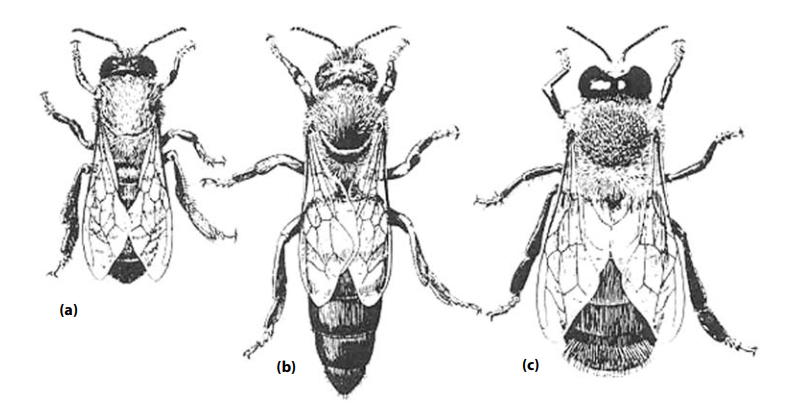
\includegraphics[width=0.75\textwidth]{assets/abejas.png}
  \caption{Castas de abejas. \cite{david_cramp}}
  \label{fig:abejas}
\end{figure}

Como se observa en la figura~\ref{fig:abejas}, las castas de abejas son las siguientes:
\begin{enumerate}
  \renewcommand\labelenumi{\alph{enumi})}
  \item \textbf{Obreras}: Estas se encargan de todas las tareas no relacionadas con la reproducción, incluyendo la construcción del panal, la recolección de polen, la producción de miel, entre otras actividades vitales para la colmena.
  \item \textbf{Reinas}: Son la única hembra completa de la colonia; su única responsabilidad es reproducirse y poner huevos.
  \item \textbf{Drones}: Similar a la reina; su única responsabilidad es reproducirse con reinas de otras colonias.
\end{enumerate}

\subsection{Temperatura de la colmena}
Una colmena debe de mantener una temperatura cercana a los 34 grados centígrados, para lograr esto pueden implementar ciertos mecanismos de regulación de temperatura. \cite{david_cramp}
Cuando las abejas necesitan elevar la temperatura, generan una capa de abejas vivas alrededor de la reina, después proceden a vibrar con el objetivo de producir calor. Para este proceso es necesario que la colmena cuente con suficiente alimento, además, se apoya del aislamiento de la colmena, ya sea natural o artificial, de modo natural, la miel y la cera son buenos aislantes. \cite{chadwick_alton_tennant_fitzmaurice_earl_2016}
Por otro lado, las abejas suelen iniciar un aleteo con sus alas para reducir la temperatura dentro de la colmena. \cite{chadwick_alton_tennant_fitzmaurice_earl_2016}

\subsection{Humedad de la colmena}
La humedad tiene un papel importante en la prevención de enfermedades dentro de la colmena, por esta razón es de importancia para las abejas controlar esta propiedad, el mecanismo que utilizan las abejas en estos casos es utilizar sus alas como ventiladores para expulsar la humedad de la colmena. \cite{chadwick_alton_tennant_fitzmaurice_earl_2016}

\subsection{Peso de la colmena}
El peso es el principal factor utilizado por los apicultores para medir la cantidad en los almacenes de miel, de manera tradicional, los apicultores intentan levantar la colmena, en caso de no ser capaces, consideran que la miel esta lista para ser extraída \cite{chadwick_alton_tennant_fitzmaurice_earl_2016}, de manera precisa, se considera una extracción cuando el almacén de miel pesa cerca a los 40kg.\cite{david_cramp}

\subsection{Enjambrado}
El evento de enjambre sucede cuando una colonia de abejas ha sobrepasado el límite físico de la colmena en la que habita, este proceso comienza con la reina engendrando nuevas reinas y drones, después de esto un enjambre de abejas y drones emigran a un nuevo posible lugar en el cual comienza una nueva colmena. \cite{chadwick_alton_tennant_fitzmaurice_earl_2016}

Uno de los principales indicadores del enjambrado es el sonido que emiten las abejas, durante este proceso comienzan a emitir un sonido de vibración, este sonido es conocido por los apicultores y es la principal fuente de información que se obtiene sobre este proceso \cite{david_cramp} \cite{chadwick_alton_tennant_fitzmaurice_earl_2016}.

\subsection{Internet e IoT}

\subsubsection{Internet}
En el contexto actual, internet se refiere a una red global con varios protocolos de conectividad que permite comunicar paquetes de datos de dispositivos, mediante un sistema de rúters, a la red. \cite{kamal_2017}

\subsubsection{Rúter, router o enrutador}
Se refiere a un dispositivo capaz de almacenar direcciones y enlaces mediante las cuales se encarga de mandar paquetes de datos.\cite{kamal_2017}

\subsubsection{Internet de las cosas (IoT)}
El termino de internet de las coas, o IOT por sus siglas en inglés (Internet of things), se refiere al concepto de entrelazar objetos físicos dentro de una red de internet, mediante componentes electrónicos y sistemas de software, con el objetivo de permitir la comunicación entre ellos y monitorear o controlar un sistema físico. \cite{kamal_2017}

\subsubsection{Arquitectura IoT}
Este concepto se refiere a la forma de estructurar u diseñar un sistema IOT y estos se dividen en capas y son 7 principales
\begin{enumerate}
  \renewcommand\labelenumi{\arabic{enumi}.}
  \item Componentes físicos: sensores y controladores.
  \item Dispositivos de conectividad.
  \item Computación perimetral (análisis de datos y procesamiento).
  \item Persistencia de datos.
  \item Abstracción de datos (acceso y manipulación).
  \item Aplicación (reportes, análisis y control).
  \item Colaboración y procesos (usuarios y procesos comerciales).
\end{enumerate}
Estas capas sirven para estructurar y definir la arquitectura del sistema IOT.\cite{kamal_2017}


\subsubsection{Sensores}
El sistema IOT interactúa con sensores, dispositivos físicos con el objetivo de adquirir datos mediante la capacidad de reaccionar a parámetros físicos como la humedad, temperatura, presión y luz y convertirla en energía eléctrica capaz de interactuar con el sistema. Durante esta interacción es posible configurar los dispositivos de manera que se ajusten a los requerimientos de la aplicación.\cite{kamal_2017}

\subsubsection{Colmenas inteligentes}
Los términos Colmenas IOT o colmenas inteligentes se refieren a la adición de un sistema IOT a una colmena apícola, esto con el objetivo de monitorear los parámetros de la colonia de abejas y hacer accesible la información de manera que pueda ser procesada para conocer el estado de la colmena. \cite{open_source_beehives_project_iaac}

\subsection{Inteligencia artificial}

\subsubsection{Sistema inteligente}
Se refiere a un concepto abstracto en el cual se define a un sistema que actúa y razona de manera humana o de manera lógica \cite{russell_norvig_2022}. Es uno de los posibles métodos para procesar datos de un sistema IOT \cite{open_source_beehives_project_iaac}.

\subsubsection{Minería de datos}
Se refiere al proceso de aplicar métodos computacionales a grandes cantidades de datos con el objetivo de revelar información nueva, no trivial y relevante \cite{fayyad1996kdd}. Esto incluye la aplicación de algoritmos específicos para la extracción de patrones, la limpieza de datos, el preprocesamiento y la extracción de características.


\subsubsection{Preprocesamiento de datos}
El preprocesamiento de datos es una etapa en la minería de datos que consiste en preparar y limpiar el conjunto de datos con el objetivo de mejorar su calidad para que sean adecuados para el análisis o modelado. Esto implica corregir valores inválidos, eliminar columnas irrelevantes, manejar valores faltantes, ajustar datos inconsistentes, entre otros \cite{statistical_modeling_in_machine_learning_2023}.

\subsubsection{Aprendizaje automático}
El aprendizaje automático, o aprendizaje maquina, es una rama de la inteligencia artificial que se centra en desarrollar algoritmos capaces de aprender automáticamente a partir de los datos y mejorar su desempeño con la experiencia, sin ser programados explícitamente. Formalmente, se dice que un programa aprende de una experiencia $E$ respecto a una clase de tareas $T$ y una medida de desempeño $P$, si su desempeño en las tareas de $T$, medida por $P$, mejora con la experiencia $E$. En otras palabras, el desempeño del algoritmo en una tarea mejora conforme gana experiencia al realizarla \cite{mitchell1997machine}.


\subsubsection{Extracción de características}
La extracción de características es una técnica de preprocesamiento de datos utilizada en el aprendizaje máquina para transformar un conjunto de datos complejos y con muchas características, en un espacio más manejable y representativo. Se utiliza cuando hay demasiadas características ya sea para un análisis efectivo o para la visualización de datos \cite{richer_coelho_2013}.

\subsubsection{Características de audio}

\begin{itemize}
  \item \textbf{Zero Crossing Rate (ZCR):} Número de veces que la señal cruza el eje cero por unidad de tiempo. Indica la frecuencia de cambios en la señal, útil para distinguir sonidos ruidosos y tonales \cite{muller2015fmp}.

  \item \textbf{RMS (Root Mean Square):} Raíz cuadrada del promedio cuadrático de las muestras; mide energía promedio de la señal, útil para comparar su intensidad relativa entre segmentos \cite{sound_quality_heyboer2010}.

  \item \textbf{Energía:} Suma de los cuadrados de las amplitudes de la señal, representa la potencia o intensidad del sonido \cite{rabiner2010fundamentals}.

  \item \textbf{Entropía de energía:} Mide la distribución y variabilidad de la energía dentro de una señal, calculada usando entropía de Shannon sobre segmentos de energía \cite{li2017audio}.

  \item \textbf{Centroide espectral:} Promedio ponderado de las frecuencias presentes en una señal, que refleja el "brillo" percibido del sonido \cite{peeters2004large}.

  \item \textbf{Dispersión espectral:} Desviación estándar de la distribución espectral alrededor del centroide, indica la extensión del contenido frecuencial \cite{peeters2004large}.

  \item \textbf{Entropía espectral:} Entropía de Shannon aplicada a la densidad espectral de potencia, mide la complejidad del espectro \cite{jiang2011spectral}.

  \item \textbf{Flujo espectral:} Cambio en el espectro de potencia entre frames consecutivos, usado para detectar transiciones y dinámica en la señal \cite{foote2000novelty}.

  \item \textbf{Rolloff espectral:} Frecuencia debajo de la cual se acumula un porcentaje dado (e.g., 85\%) de la energía espectral, útil para distinguir sonidos agudos de graves \cite{tzanetakis2002musical}.

  \item \textbf{MFCC (1 a 13):} Coeficientes cepstrales calculados sobre la escala de frecuencias Mel, que modelan el timbre y la estructura espectral, ampliamente usados en reconocimiento de voz y análisis musical \cite{davis1980tassp}.
\end{itemize}




\section{Trabajos relacionados}
La adición de tecnologías de internet de las cosas (IoT) en la apicultura ha significado un cambio revolucionario a comparación de las prácticas tradicionales, aumentando la eficiencia, productividad y escalabilidad. Estas tecnologías involucran el uso de diferentes sistemas interconectados, incluyendo sensores, microcontroladores y software, con el objetivo de ayudar a monitorear y administrar las actividades apícolas en tiempo real.
En este capítulo se exploran las aplicaciones relevantes en las cuales se han desarrollado las aplicaciones de IoT en el monitoreo de colmenas apícolas, con el objetivo de dar seguimiento a la salud y actividad de las colonias de abejas, proveyendo así información de la colmena, incluyendo parámetros como temperatura, humedad, peso y acústica que ayudan a los apicultores a mantener colonias saludables y tomar decisiones acordes a la información en tiempo real.
La arquitectura de sistemas IoT para monitoreo de colmenas involucra varios componentes clave, incluyendo nodos de sensores, sistemas de transmisión de datos, sistemas de energía y el componente de procesamiento de datos. En este capítulo se examinan las prácticas utilizadas para implementar estos sistemas.

\subsection{Embedded Software for IoT Bee Hive Monitoring Node}
Este artículo presenta un sistema embebido para monitoreo de variables relevantes; se propone un sistema que tiene las capacidades de monitorear humedad, temperatura, peso y audio. Sin embargo, solo se detalla la implementación del monitoreo de humedad y temperatura. Para este sistema se utilizó el sensor SHT21~\cite{sht21} para la medición de temperatura y humedad.~\cite{vidrascu_svasta_2017a}  
El sistema está construido alrededor del componente ESP8266 que integra un microcontrolador Tensilica L106 de 32 bits en conjunto con el módulo transmisor Wi-Fi que integra circuitos de radiofrecuencia y es capaz de transmitir datos mediante interfaces digitales como SPI, I2C, y UART. Además, el módulo ESP8266 cuenta con tres modos de operación: activo, dormido y dormido profundo, los cuales son aprovechados por el sistema para optimizar el uso de energía.~\cite{vidrascu_svasta_2017a}

\subsection{A Smart Sensor-Based Measurement System for Advanced Bee Hive Monitoring}
Este sistema desarrolla un monitoreo de parámetros relevantes para la colmena, incluyendo peso, sonido, temperatura, humedad y CO$_2$.~\cite{cecchi_spinsante_terenzi_orcioni_2020}  
Es modular y se compone de dos módulos principales:  
\begin{itemize}
    \item \textbf{Módulo Abeja}: Raspberry Pi 3B~\cite{buy_raspberry_pi3_model_b}, tarjeta de sonido UCA22~\cite{behringer_uca222}, micrófonos ADMP401 MEMS~\cite{admp401_datasheet}, sensores DHT22~\cite{liu}, células de carga TAL220~\cite{loadcell_tal220_sparkfun} con HX711~\cite{hx711_sparkfun} y sensor de CO$_2$ TL6615~\cite{t6615_telaire}.
    \item \textbf{Módulo Reina}: Raspberry Pi 3B, sensores DHT22 y un puente 5G (no especificado) utilizado para comunicarse con el servidor remoto.~\cite{cecchi_spinsante_terenzi_orcioni_2020}
\end{itemize}  
Este artículo se energiza mediante una conexión a la red eléctrica, los módulos Reina y Abeja consumen 4 y 4.2 watts respectivamente.~\cite{cecchi_spinsante_terenzi_orcioni_2020}

\subsection{High Reliability Wireless Sensor Node for Bee Hive Monitoring}
Este sistema está diseñado para condiciones de entre -20 a 60 °C con una arquitectura modular que permite intercambiar sensores mediante interfaz I2C.~\cite{vidrascu_svasta_vladescu_2016}  
Incluye sensores SHT21, sistema HX711 con células de carga, sensor de inclinación DMA08 y micrófono MP34DT05-A.~\cite{vidrascu_svasta_vladescu_2016}  
Además, utiliza un módulo ESP8266 serie 32-bit a 80MHz para conexión Wi-Fi directa.~\cite{vidrascu_svasta_vladescu_2016}  
En cuanto a la energía, se emplean supercapacitores XV de Eaton~\cite{supercapacitor_xv_eaton} junto con paneles solares (no especificados) y un convertidor step up.~\cite{vidrascu_svasta_vladescu_2016}

\subsection{Bee Swarm Activity Acoustic Classification for an IoT-Based Farm Service}
Este sistema utiliza un micrófono TDK InvenSense ICS-40300 y una placa Atmel ATmega32U4 sobre la colmena, procesando los datos en un servidor remoto.~\cite{zgank_2019}  
El procesamiento de datos acústicos tiene como objetivo la detección de enjambres, utilizando datos del Open Source Beehives Project (OSBP)~\cite{open_source_beehives_project_iaac}. Se aplican métodos MFCC y LPC para extracción de características y HMM/GMM para clasificación.~\cite{zgank_2019}

\subsection{Maintenance-free IoT Gateway Design for Bee Hive Monitoring}
Este módulo recopila información con sensores SHT21, MPL3115A2~\cite{nxp_mpl3115a2}, TSL2561~\cite{tsl2561_adafruit}, HX711, VEML6075~\cite{adafruit_veml6075} y GP2Y1010AU0F~\cite{vidrascu_svasta_2017b}.~\cite{vidrascu_svasta_2017b}  
Para transmisión de datos se utiliza un ESP8266-12 (A.I.Thinker) y un módem A6 GSM/GPRS (no en bib).~\cite{vidrascu_svasta_2017b}  
El sistema obtiene energía de paneles solares (no especificados) con reguladores LT3652~\cite{lt3652_datasheet} y LTC3652~\cite{ltc3652_datasheet}.~\cite{vidrascu_svasta_2017b}

\subsection{A Pi-Based IoT System Design}
Este sistema integra la suite de sensores GrovePi: humedad, temperatura, GPS, sonido e imágenes térmicas.~\cite{chen_chien_hsu_jing_lin_lin_2020}  
Implementa múltiples módulos Wi-Fi conectados a un módem independiente con conexión a red móvil.~\cite{chen_chien_hsu_jing_lin_lin_2020}  
Se alimenta con una batería de 10000 mAh (180000 J a 5V), con autonomía de 27–33 h.~\cite{chen_chien_hsu_jing_lin_lin_2020}

\subsection{Conclusión}
A lo largo de este capítulo, se han explorado diversas arquitecturas y tecnologías utilizadas en estos sistemas, destacando los componentes esenciales como los nodos de sensores y los sistemas de transmisión de datos, así como las soluciones innovadoras para el manejo de energía y el procesamiento de datos.
\begin{itemize}
    \item \textbf{Nodos de Sensores}: Los sistemas presentados varían en complejidad, pero todos incluyen sensores de temperatura, humedad, peso y acústica.
    \item \textbf{Sistemas de Transmisión de Datos}: Predomina el uso del módulo ESP8266, con casos que incorporan GSM/GPRS.
    \item \textbf{Manejo de Energía}: Paneles solares, baterías y supercapacitores son las soluciones más comunes.
    \item \textbf{Procesamiento de Datos}: Se emplean MFCC, LPC, HMM y GMM en clasificación de eventos acústicos.
\end{itemize}
La adición de tecnologías de internet de las cosas (IoT) en la apicultura ha significado un cambio revolucionario a comparación de las prácticas tradicionales, aumentando la eficiencia, productividad y escalabilidad. Estas tecnologías involucran el uso de diferentes sistemas interconectados, incluyendo sensores, microcontroladores y software, con el objetivo de ayudar a monitorear y administrar las actividades apícolas en tiempo real.
En este capítulo se exploran las aplicaciones relevantes en las cuales se han desarrollado las aplicaciones de IoT en el monitoreo de colmenas apícolas, con el objetivo de dar seguimiento a la salud y actividad de las colonias de abejas, proveyendo así información de la colmena, incluyendo parámetros como temperatura, humedad, peso y acústica que ayudan a los apicultores a mantener colonias saludables y tomar decisiones acordes a la información en tiempo real.
La arquitectura de sistemas IoT para monitoreo de colmenas involucra varios componentes clave, incluyendo nodos de sensores, sistemas de transmisión de datos, sistemas de energía y el componente de procesamiento de datos. En este capítulo se examinan las prácticas utilizadas para implementar estos sistemas.

\subsection{Embedded Software for IoT Bee Hive Monitoring Node}
Este artículo presenta un sistema embebido para monitoreo de variables relevantes; se propone un sistema que tiene las capacidades de monitorear humedad, temperatura, peso y audio. Sin embargo, no se implementó el monitoreo de peso y audio. Para este sistema se utilizó el sensor SHT21~\cite{sht21} para la medición de temperatura y humedad.~\cite{vidrascu_svasta_2017a}  
El sistema está construido alrededor del componente ESP8266 que integra un microcontrolador Tensilica L106 32-bit en conjunto con el módulo transmisor Wi-Fi que integra circuitos de radio frecuencia y es capaz de transmitir datos mediante interfaces digitales como SPI, I2C, y UART. Además, el módulo ESP8266 cuenta con tres modos de operación: activo, dormido y dormido profundo, los cuales son aprovechados por el sistema para optimizar el uso de energía.~\cite{vidrascu_svasta_2017a}

\subsection{A Smart Sensor-Based Measurement System for Advanced Bee Hive Monitoring}
Este sistema desarrolla un monitoreo de parámetros relevantes para la colmena, incluyendo peso, sonido, temperatura, humedad y CO$_2$.~\cite{cecchi_spinsante_terenzi_orcioni_2020}  
Es modular y se compone de dos módulos principales:  
\begin{itemize}
    \item \textbf{Módulo Abeja}: Raspberry Pi 3B~\cite{buy_raspberry_pi3_model_b}, tarjeta de sonido UCA22~\cite{behringer_uca222}, micrófonos ADMP401 MEMS~\cite{admp401_datasheet}, sensores DHT22~\cite{liu}, células de carga TAL220~\cite{loadcell_tal220_sparkfun} con HX711~\cite{hx711_sparkfun} y sensor de CO$_2$ TL6615~\cite{t6615_telaire}.
    \item \textbf{Módulo Reina}: Raspberry Pi 3B, sensores DHT22 y un puente 5G (no especificado) utilizado para comunicarse con el servidor remoto.~\cite{cecchi_spinsante_terenzi_orcioni_2020}
\end{itemize}  
Este artículo se energiza mediante una conexión a la red eléctrica, los módulos Reina y Abeja consumen 4 y 4.2 watts respectivamente.~\cite{cecchi_spinsante_terenzi_orcioni_2020}

\subsection{High Reliability Wireless Sensor Node for Bee Hive Monitoring}
Este sistema está diseñado para condiciones de entre -20 a 60 °C con una arquitectura modular que permite intercambiar sensores mediante interfaz I2C.~\cite{vidrascu_svasta_vladescu_2016}  
Incluye sensores SHT21, sistema HX711 con células de carga, sensor de inclinación DMA08 y micrófono MP34DT05-A.~\cite{vidrascu_svasta_vladescu_2016}  
Además, utiliza un módulo ESP8266 serie 32-bit a 80MHz para conexión Wi-Fi directa.~\cite{vidrascu_svasta_vladescu_2016}  
En cuanto a la energía, se emplean supercapacitores XV de Eaton~\cite{supercapacitor_xv_eaton} junto con paneles solares (no especificados) y un convertidor step up.~\cite{vidrascu_svasta_vladescu_2016}

\subsection{Bee Swarm Activity Acoustic Classification for an IoT-Based Farm Service}
Este sistema utiliza un micrófono TDK InvenSense ICS-40300 y una placa Atmel ATmega32U4 sobre la colmena, procesando los datos en un servidor remoto.~\cite{zgank_2019}  
El procesamiento de datos acústicos tiene como objetivo la detección de enjambres, utilizando datos del Open Source Beehives Project (OSBP)~\cite{open_source_beehives_project_iaac}. Se aplican métodos MFCC y LPC para extracción de características y HMM/GMM para clasificación.~\cite{zgank_2019}

\subsection{Maintenance-free IoT Gateway Design for Bee Hive Monitoring}
Este módulo recopila información con sensores SHT21, MPL3115A2~\cite{nxp_mpl3115a2}, TSL2561~\cite{tsl2561_adafruit}, HX711, VEML6075~\cite{adafruit_veml6075} y GP2Y1010AU0F~\cite{vidrascu_svasta_2017b}.~\cite{vidrascu_svasta_2017b}  
Para transmisión de datos se utiliza un ESP8266-12 (A.I.Thinker) y un módem A6 GSM/GPRS (no en bib).~\cite{vidrascu_svasta_2017b}  
El sistema obtiene energía de paneles solares (no especificados) con reguladores LT3652~\cite{lt3652_datasheet} y LTC3652~\cite{ltc3652_datasheet}.~\cite{vidrascu_svasta_2017b}

\subsection{A Pi-Based IoT System Design}
Este sistema integra la suite de sensores GrovePi: humedad, temperatura, GPS, sonido e imágenes térmicas.~\cite{chen_chien_hsu_jing_lin_lin_2020}  
Implementa múltiples módulos Wi-Fi conectados a un módem independiente con conexión a red móvil.~\cite{chen_chien_hsu_jing_lin_lin_2020}  
Se alimenta con una batería de 10000 mAh (180000 J a 5V), con autonomía de 27–33 h.~\cite{chen_chien_hsu_jing_lin_lin_2020}

\subsection{Conclusión}
A lo largo de este capítulo, se han explorado diversas arquitecturas y tecnologías utilizadas en estos sistemas, destacando los componentes esenciales como los nodos de sensores y los sistemas de transmisión de datos, así como las soluciones innovadoras para el manejo de energía y el procesamiento de datos.
\begin{itemize}
    \item \textbf{Nodos de Sensores}: Los sistemas presentados varían en complejidad, pero todos incluyen sensores de temperatura, humedad, peso y acústica.
    \item \textbf{Sistemas de Transmisión de Datos}: Predomina el uso del módulo ESP8266, con casos que incorporan GSM/GPRS.
    \item \textbf{Manejo de Energía}: Paneles solares, baterías y supercapacitores son las soluciones más comunes.
    \item \textbf{Procesamiento de Datos}: Se emplean MFCC, LPC, HMM y GMM en clasificación de eventos acústicos.
\end{itemize}


\section{Métodos y herramientas}
\subsection{Sensor DHT22}

El sensor DHT22 mide temperatura y humedad. Se conecta de la siguiente manera:
\begin{figure}[!ht]
    \centering
    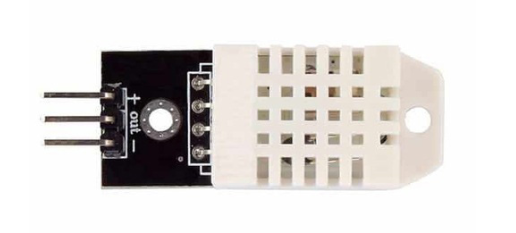
\includegraphics[width=0.4\textwidth]{assets/metodos_herramientas/dht22.png}
    \caption{Sensor DHT22.}
    \label{fig:dht22}
\end{figure}
\begin{itemize}
    \item VCC a 3.3--6 V.
    \item OUT a un pin digital con protocolo 1-wire.
    \item GND a tierra.
\end{itemize}

\begin{figure}[!ht]
    \centering
    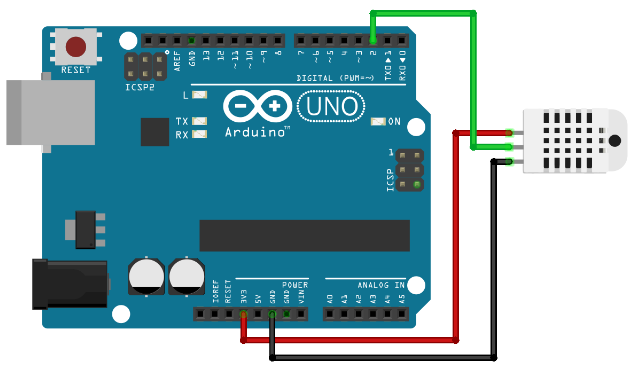
\includegraphics[width=0.5\textwidth]{assets/metodos_herramientas/arduino_dht22.png}
    \caption{Conexión del sensor DHT22 a Arduino.}
    \label{fig:arduino_dht22}
\end{figure}

\paragraph{Herramientas de software}
\begin{itemize}
    \item Arduino IDE 2.2.1 en Windows 10.
    \item Librerías de Adafruit: \texttt{DHT sensor library} y \texttt{Adafruit Unified Sensor}.
\end{itemize}

\subsection{Celda de carga y módulo HX711}
Las celdas de carga son los sensores que recolectan información sobre el peso de una carga aplicada sobre los mismos. Los sensores a utilizar son equivalentes a los de la ilustración 3, cuentan con 4 cables y 4 orificios roscados para fijar la celda, así como una imagen indicativa de la dirección de la carga.

\begin{figure}[!ht]
    \centering
    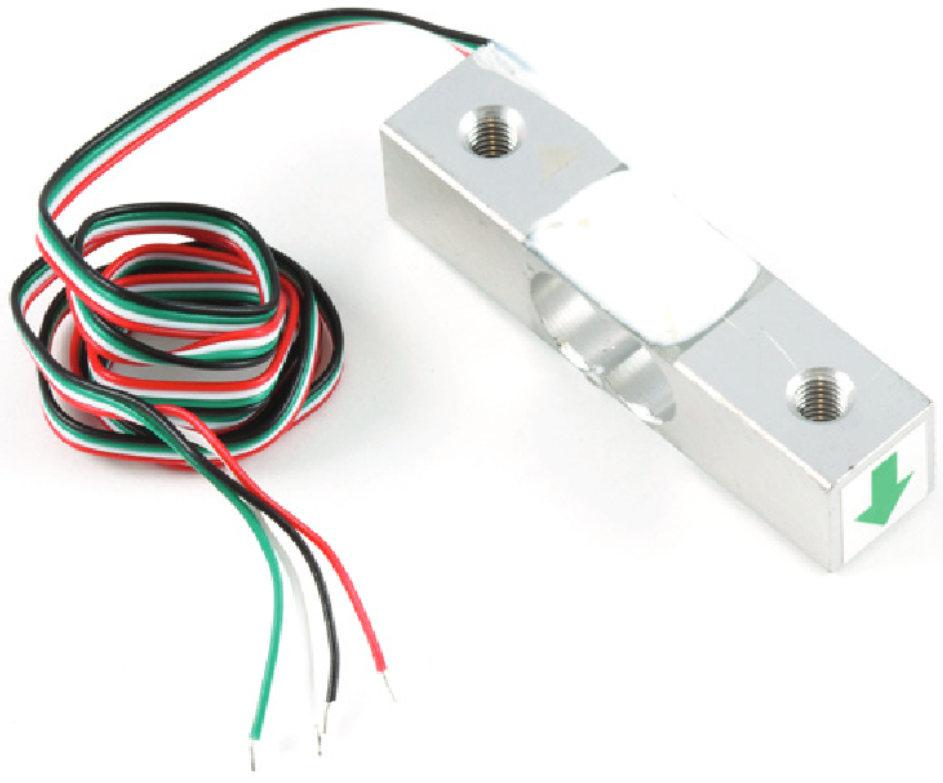
\includegraphics[width=0.5\textwidth]{assets/metodos_herramientas/celda_carga.png}
    \caption{Celda de carga.}
    \label{fig:celda_carga}
\end{figure}
\newpage

El módulo HX711 es una placa electrónica que funciona como interfaz entre una placa Arduino y una celda de carga. Este se muestra en la ilustración \ref{fig:hx711}. El módulo HX711 es un convertidor analógico a digital (ADC) de 24 bits, diseñado específicamente para aplicaciones de pesaje y medición de fuerza. Permite leer las señales analógicas de la celda de carga y convertirlas en valores digitales que pueden ser procesados por un microcontrolador como Arduino.

\begin{figure}[!ht]
    \centering
    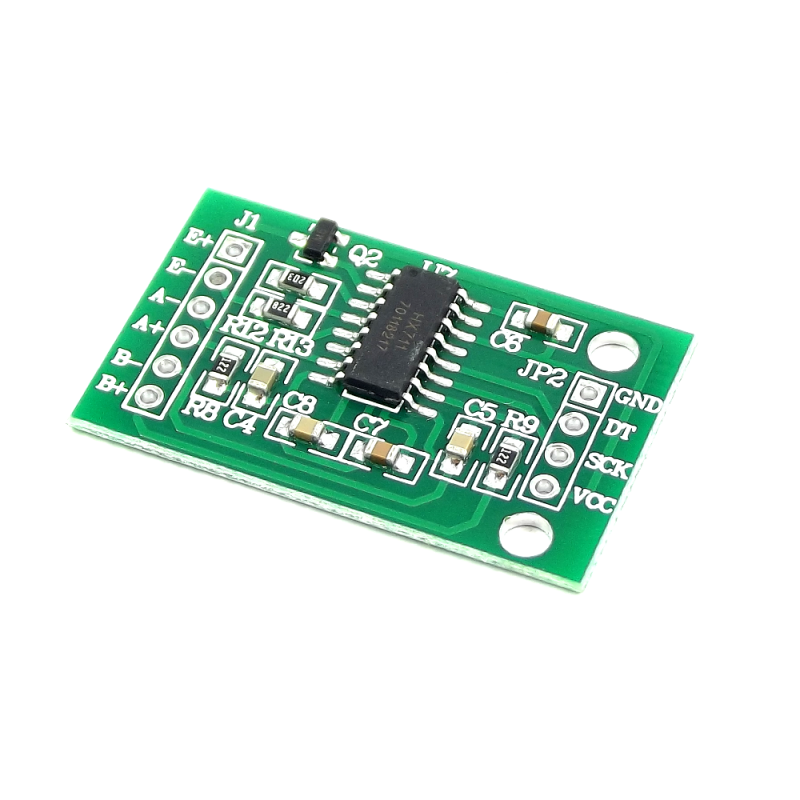
\includegraphics[width=0.5\textwidth]{assets/metodos_herramientas/hx711.png}
    \caption{Módulo HX711.}
    \label{fig:hx711}
\end{figure}
Las conexiones se realizan de acuerdo a las tablas \ref{tab:conexiones_celda_hx711} y \ref{tab:conexiones_hx711_arduino}. La celda de carga se conecta al módulo HX711, y este último se conecta a la placa Arduino. El módulo HX711 requiere una alimentación de 5 V y tiene dos pines de salida: uno para la señal de datos (DT) y otro para el reloj (SCK).
\begin{table}[!ht]
    \centering
    \rowcolors{2}{gray!10}{white}
    \begin{tabularx}{\textwidth}{>{\bfseries}X X}
        \toprule
        \textbf{COLOR DEL CABLE} & \textbf{CONECCIÓN EN MÓDULO} \\
        \midrule
        ROJO                     & E+                           \\
        NEGRO                    & E-                           \\
        BLANCO                   & A-                           \\
        VERDE                    & A+                           \\
        \bottomrule
    \end{tabularx}
    \caption{\textit{conexiones celda-HX711}}
\end{table}
\begin{table}[!ht]
    \centering
    \rowcolors{2}{gray!10}{white}
    \begin{tabularx}{\textwidth}{>{\bfseries}X X}
        \toprule
        \textbf{PIN HX711} & \textbf{CONECCIÓN EN ARDUINO} \\
        \midrule
        GND                & GND                           \\
        DT                 & A1                            \\
        SCK                & A0                            \\
        VCC                & 5 V                           \\
        \bottomrule
    \end{tabularx}
    \caption{\textit{conexiones HX711-Arduino}}
\end{table}
\newpage

\paragraph{Ejemplo de código HX711}\mbox{}

\begin{lstlisting}[language=C++, caption={Ejemplo de código HX711}, label={lst:ejemplo_hx711}]
#include "HX711.h"
const int DOUT = A1;
const int CLK = A0;
HX711 balanza;

void setup() {
  Serial.begin(9600);
  balanza.begin(DOUT, CLK);
  balanza.set_scale(439430.25);
  balanza.tare();
}

void loop() {
  Serial.println(balanza.get_units());
  delay(1000);
}
\end{lstlisting}

\subsection{Controlador ESP32}
El ESP32 integra Wi-Fi y Bluetooth en un solo chip con bajo consumo en modo Deep Sleep (~10 \textmu{}A a 3.3 V).
\begin{itemize}
    \item Procesador: Xtensa LX6, 32 bits, hasta 240 MHz.
    \item RAM: 520 KB SRAM.
\end{itemize}

Para utilizar el controlador con el Arduino IDE2.0 es necesario agregar el siguiente paquete a Additional Boards Manager como se muestra en la figura  \ref{fig:arduino_placas} y el código \ref{lst:esp32_boards_manager}.
\begin{lstlisting}[language=, label={lst:esp32_boards_manager}, caption={URL para Boards Manager de ESP32}]
https://raw.githubusercontent.com/espressif/arduino-esp32/gh-pages/package_esp32_index.json
\end{lstlisting}

\newpage

\begin{figure}[!ht]
    \centering
    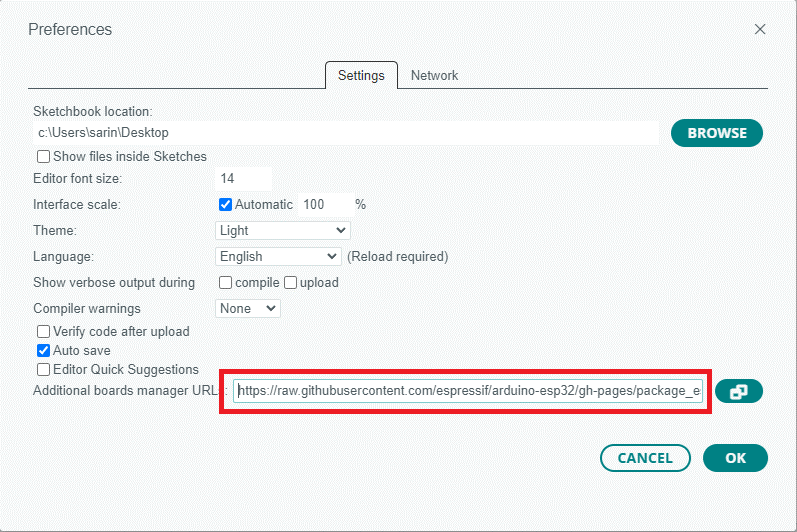
\includegraphics[width=0.75\textwidth]{assets/metodos_herramientas/arduino_placas.png}
    \caption{Selección de placas ESP32 en Arduino IDE.}
    \label{fig:arduino_placas}
\end{figure}

El siguiente paso es instalar los controladores para la placa ESP32, se muestra en la figura  \ref{fig:arduino_install_esp32}.

\begin{figure}[!ht]
    \centering
    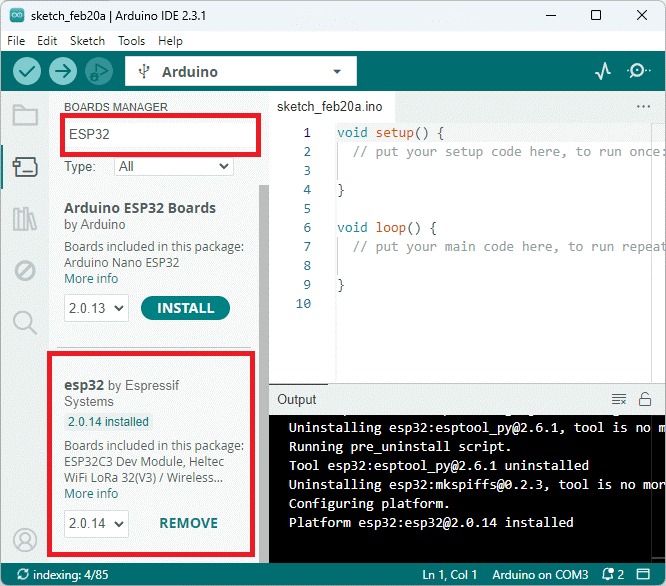
\includegraphics[width=0.75\textwidth]{assets/metodos_herramientas/arduino_install_esp32.png}
    \caption{Instalación del soporte para ESP32 en Arduino IDE.}
    \label{fig:arduino_install_esp32}
\end{figure}

\newpage

Código de prueba:
\begin{lstlisting}[language=C++, label={lst:esp32_blink}, caption={Ejemplo de código de parpadeo de LED en ESP32}]
#include <Arduino.h>
#define LED 2
void setup() {
  Serial.begin(115200);
  pinMode(LED, OUTPUT);
}
void loop() {
  digitalWrite(LED, HIGH);
  delay(1000);
  digitalWrite(LED, LOW);
  delay(1000);
}
\end{lstlisting}

\subsection{Micrófono INMP441}
\begin{figure}[!ht]
    \centering
    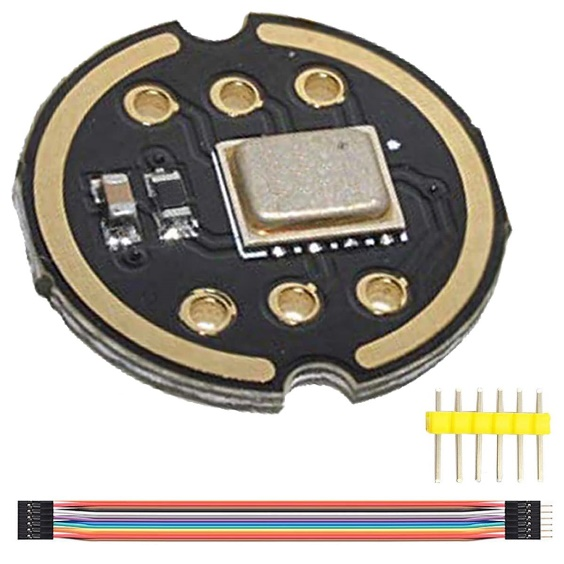
\includegraphics[width=0.75\textwidth]{assets/metodos_herramientas/inmp441.png}
    \caption{Módulo de micrófono INMP441.}
    \label{fig:inmp441}
\end{figure}

El sensor INMP441 es un micrófono multidireccional que utiliza el protocolo I2S~\cite{keysight_i2s_blog} para transferencia de audio, de la misma manera que, y como se mencionó en los trabajos relacionados, el dispositivo INMP401 es utilizado con el controlador ESP8266, el dispositivo INMP441 es comúnmente utilizado con el dispositivo ESP32, principalmente por su compatibilidad mediante el protocolo I2S. El módulo INMP441 se muestra en la figura  7~\cite{inmp441_datasheet}.


\chapter{Estado del arte}
\label{chap:estado_arte}

\section{Marco teórico}
\subsection{Introducción}
La implementación de la infraestructura de telecomunicaciones ha transformado numerosos aspectos de la vida cotidiana y el ámbito industrial, dando lugar a innovaciones que facilitan la comunicación y el control de diversos sistemas. Uno de estos avances es el Internet de las Cosas (IoT), que conecta objetos físicos a la red, permitiendo su monitoreo y control a través de dispositivos electrónicos y software. En este contexto, en el área de la apicultura se han adoptado tecnologías IoT para mejorar la gestión y el monitoreo de las colmenas, creando lo que se conoce como colmenas inteligentes.

En este capítulo se ofrece un marco teórico sobre los conceptos clave del internet, IoT y su aplicación en la apicultura. Se explora la arquitectura IoT, desglosada en sus siete capas fundamentales, y se examina la interacción de los sensores en estos sistemas. Además, se profundiza en el uso de IoT en las colmenas, destacando su capacidad para monitorear parámetros críticos como la temperatura, la humedad y el peso de la colmena, así como para detectar el enjambrado a través del análisis de sonidos específicos. También se proporciona una visión general sobre la inteligencia artificial y su potencial integración en sistemas IoT para optimizar el control y análisis de datos en la apicultura.
\subsection{Apicultura}
Se refiere a la crianza y explotación de abejas, de las cuales se obtienen productos como miel, cera y polen, y que al mismo tiempo realizan el servicio de polinización de plantas.

\subsection{Abejas}
Se refiere a un insecto social que durante su ciclo de vida se encarga de producir miel, cera y panal y polinizar plantas para apoyarlas en su reproducción, por lo cual se les considera de los insectos más importantes del planeta.  \cite{david_cramp}

\subsection{Colmena}
Una abeja no puede sobrevivir de manera individual, una abeja obrera no se puede reproducir y una abeja reina no puede construir o mantener una colmena ya que la estructura social de las abejas requiere de a las obreras, las reinas y los drones para sobrevivir, por lo cual se considera a la misma como un organismo independiente. \cite{david_cramp} En la figura~\ref{fig:abejas} se muestra una imagen ilustrativa de las 3 castas de abeja.

\begin{figure}[htbp]
  \centering
  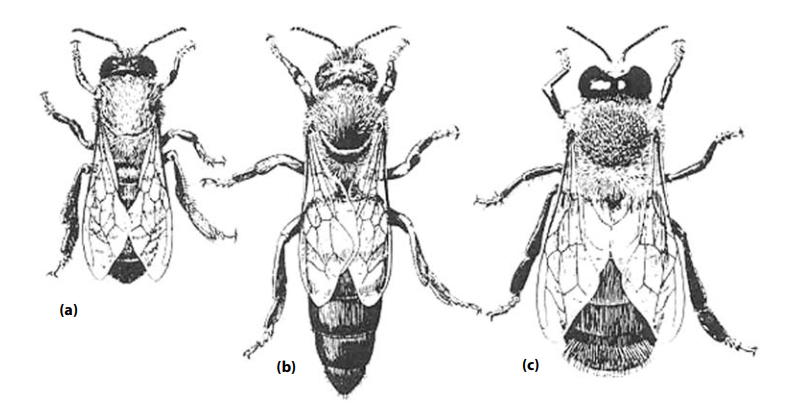
\includegraphics[width=0.75\textwidth]{assets/abejas.png}
  \caption{Castas de abejas. \cite{david_cramp}}
  \label{fig:abejas}
\end{figure}

Como se observa en la figura~\ref{fig:abejas}, las castas de abejas son las siguientes:
\begin{enumerate}
  \renewcommand\labelenumi{\alph{enumi})}
  \item \textbf{Obreras}: Estas se encargan de todas las tareas no relacionadas con la reproducción, incluyendo la construcción del panal, la recolección de polen, la producción de miel, entre otras actividades vitales para la colmena.
  \item \textbf{Reinas}: Son la única hembra completa de la colonia; su única responsabilidad es reproducirse y poner huevos.
  \item \textbf{Drones}: Similar a la reina; su única responsabilidad es reproducirse con reinas de otras colonias.
\end{enumerate}

\subsection{Temperatura de la colmena}
Una colmena debe de mantener una temperatura cercana a los 34 grados centígrados, para lograr esto pueden implementar ciertos mecanismos de regulación de temperatura. \cite{david_cramp}
Cuando las abejas necesitan elevar la temperatura, generan una capa de abejas vivas alrededor de la reina, después proceden a vibrar con el objetivo de producir calor. Para este proceso es necesario que la colmena cuente con suficiente alimento, además, se apoya del aislamiento de la colmena, ya sea natural o artificial, de modo natural, la miel y la cera son buenos aislantes. \cite{chadwick_alton_tennant_fitzmaurice_earl_2016}
Por otro lado, las abejas suelen iniciar un aleteo con sus alas para reducir la temperatura dentro de la colmena. \cite{chadwick_alton_tennant_fitzmaurice_earl_2016}

\subsection{Humedad de la colmena}
La humedad tiene un papel importante en la prevención de enfermedades dentro de la colmena, por esta razón es de importancia para las abejas controlar esta propiedad, el mecanismo que utilizan las abejas en estos casos es utilizar sus alas como ventiladores para expulsar la humedad de la colmena. \cite{chadwick_alton_tennant_fitzmaurice_earl_2016}

\subsection{Peso de la colmena}
El peso es el principal factor utilizado por los apicultores para medir la cantidad en los almacenes de miel, de manera tradicional, los apicultores intentan levantar la colmena, en caso de no ser capaces, consideran que la miel esta lista para ser extraída \cite{chadwick_alton_tennant_fitzmaurice_earl_2016}, de manera precisa, se considera una extracción cuando el almacén de miel pesa cerca a los 40kg.\cite{david_cramp}

\subsection{Enjambrado}
El evento de enjambre sucede cuando una colonia de abejas ha sobrepasado el límite físico de la colmena en la que habita, este proceso comienza con la reina engendrando nuevas reinas y drones, después de esto un enjambre de abejas y drones emigran a un nuevo posible lugar en el cual comienza una nueva colmena. \cite{chadwick_alton_tennant_fitzmaurice_earl_2016}

Uno de los principales indicadores del enjambrado es el sonido que emiten las abejas, durante este proceso comienzan a emitir un sonido de vibración, este sonido es conocido por los apicultores y es la principal fuente de información que se obtiene sobre este proceso \cite{david_cramp} \cite{chadwick_alton_tennant_fitzmaurice_earl_2016}.

\subsection{Internet e IoT}

\subsubsection{Internet}
En el contexto actual, internet se refiere a una red global con varios protocolos de conectividad que permite comunicar paquetes de datos de dispositivos, mediante un sistema de rúters, a la red. \cite{kamal_2017}

\subsubsection{Rúter, router o enrutador}
Se refiere a un dispositivo capaz de almacenar direcciones y enlaces mediante las cuales se encarga de mandar paquetes de datos.\cite{kamal_2017}

\subsubsection{Internet de las cosas (IoT)}
El termino de internet de las coas, o IOT por sus siglas en inglés (Internet of things), se refiere al concepto de entrelazar objetos físicos dentro de una red de internet, mediante componentes electrónicos y sistemas de software, con el objetivo de permitir la comunicación entre ellos y monitorear o controlar un sistema físico. \cite{kamal_2017}

\subsubsection{Arquitectura IoT}
Este concepto se refiere a la forma de estructurar u diseñar un sistema IOT y estos se dividen en capas y son 7 principales
\begin{enumerate}
  \renewcommand\labelenumi{\arabic{enumi}.}
  \item Componentes físicos: sensores y controladores.
  \item Dispositivos de conectividad.
  \item Computación perimetral (análisis de datos y procesamiento).
  \item Persistencia de datos.
  \item Abstracción de datos (acceso y manipulación).
  \item Aplicación (reportes, análisis y control).
  \item Colaboración y procesos (usuarios y procesos comerciales).
\end{enumerate}
Estas capas sirven para estructurar y definir la arquitectura del sistema IOT.\cite{kamal_2017}


\subsubsection{Sensores}
El sistema IOT interactúa con sensores, dispositivos físicos con el objetivo de adquirir datos mediante la capacidad de reaccionar a parámetros físicos como la humedad, temperatura, presión y luz y convertirla en energía eléctrica capaz de interactuar con el sistema. Durante esta interacción es posible configurar los dispositivos de manera que se ajusten a los requerimientos de la aplicación.\cite{kamal_2017}

\subsubsection{Colmenas inteligentes}
Los términos Colmenas IOT o colmenas inteligentes se refieren a la adición de un sistema IOT a una colmena apícola, esto con el objetivo de monitorear los parámetros de la colonia de abejas y hacer accesible la información de manera que pueda ser procesada para conocer el estado de la colmena. \cite{open_source_beehives_project_iaac}

\subsection{Inteligencia artificial}

\subsubsection{Sistema inteligente}
Se refiere a un concepto abstracto en el cual se define a un sistema que actúa y razona de manera humana o de manera lógica \cite{russell_norvig_2022}. Es uno de los posibles métodos para procesar datos de un sistema IOT \cite{open_source_beehives_project_iaac}.

\subsubsection{Minería de datos}
Se refiere al proceso de aplicar métodos computacionales a grandes cantidades de datos con el objetivo de revelar información nueva, no trivial y relevante \cite{fayyad1996kdd}. Esto incluye la aplicación de algoritmos específicos para la extracción de patrones, la limpieza de datos, el preprocesamiento y la extracción de características.


\subsubsection{Preprocesamiento de datos}
El preprocesamiento de datos es una etapa en la minería de datos que consiste en preparar y limpiar el conjunto de datos con el objetivo de mejorar su calidad para que sean adecuados para el análisis o modelado. Esto implica corregir valores inválidos, eliminar columnas irrelevantes, manejar valores faltantes, ajustar datos inconsistentes, entre otros \cite{statistical_modeling_in_machine_learning_2023}.

\subsubsection{Aprendizaje automático}
El aprendizaje automático, o aprendizaje maquina, es una rama de la inteligencia artificial que se centra en desarrollar algoritmos capaces de aprender automáticamente a partir de los datos y mejorar su desempeño con la experiencia, sin ser programados explícitamente. Formalmente, se dice que un programa aprende de una experiencia $E$ respecto a una clase de tareas $T$ y una medida de desempeño $P$, si su desempeño en las tareas de $T$, medida por $P$, mejora con la experiencia $E$. En otras palabras, el desempeño del algoritmo en una tarea mejora conforme gana experiencia al realizarla \cite{mitchell1997machine}.


\subsubsection{Extracción de características}
La extracción de características es una técnica de preprocesamiento de datos utilizada en el aprendizaje máquina para transformar un conjunto de datos complejos y con muchas características, en un espacio más manejable y representativo. Se utiliza cuando hay demasiadas características ya sea para un análisis efectivo o para la visualización de datos \cite{richer_coelho_2013}.

\subsubsection{Características de audio}

\begin{itemize}
  \item \textbf{Zero Crossing Rate (ZCR):} Número de veces que la señal cruza el eje cero por unidad de tiempo. Indica la frecuencia de cambios en la señal, útil para distinguir sonidos ruidosos y tonales \cite{muller2015fmp}.

  \item \textbf{RMS (Root Mean Square):} Raíz cuadrada del promedio cuadrático de las muestras; mide energía promedio de la señal, útil para comparar su intensidad relativa entre segmentos \cite{sound_quality_heyboer2010}.

  \item \textbf{Energía:} Suma de los cuadrados de las amplitudes de la señal, representa la potencia o intensidad del sonido \cite{rabiner2010fundamentals}.

  \item \textbf{Entropía de energía:} Mide la distribución y variabilidad de la energía dentro de una señal, calculada usando entropía de Shannon sobre segmentos de energía \cite{li2017audio}.

  \item \textbf{Centroide espectral:} Promedio ponderado de las frecuencias presentes en una señal, que refleja el "brillo" percibido del sonido \cite{peeters2004large}.

  \item \textbf{Dispersión espectral:} Desviación estándar de la distribución espectral alrededor del centroide, indica la extensión del contenido frecuencial \cite{peeters2004large}.

  \item \textbf{Entropía espectral:} Entropía de Shannon aplicada a la densidad espectral de potencia, mide la complejidad del espectro \cite{jiang2011spectral}.

  \item \textbf{Flujo espectral:} Cambio en el espectro de potencia entre frames consecutivos, usado para detectar transiciones y dinámica en la señal \cite{foote2000novelty}.

  \item \textbf{Rolloff espectral:} Frecuencia debajo de la cual se acumula un porcentaje dado (e.g., 85\%) de la energía espectral, útil para distinguir sonidos agudos de graves \cite{tzanetakis2002musical}.

  \item \textbf{MFCC (1 a 13):} Coeficientes cepstrales calculados sobre la escala de frecuencias Mel, que modelan el timbre y la estructura espectral, ampliamente usados en reconocimiento de voz y análisis musical \cite{davis1980tassp}.
\end{itemize}




\section{Trabajos relacionados}
La adición de tecnologías de internet de las cosas (IoT) en la apicultura ha significado un cambio revolucionario a comparación de las prácticas tradicionales, aumentando la eficiencia, productividad y escalabilidad. Estas tecnologías involucran el uso de diferentes sistemas interconectados, incluyendo sensores, microcontroladores y software, con el objetivo de ayudar a monitorear y administrar las actividades apícolas en tiempo real.
En este capítulo se exploran las aplicaciones relevantes en las cuales se han desarrollado las aplicaciones de IoT en el monitoreo de colmenas apícolas, con el objetivo de dar seguimiento a la salud y actividad de las colonias de abejas, proveyendo así información de la colmena, incluyendo parámetros como temperatura, humedad, peso y acústica que ayudan a los apicultores a mantener colonias saludables y tomar decisiones acordes a la información en tiempo real.
La arquitectura de sistemas IoT para monitoreo de colmenas involucra varios componentes clave, incluyendo nodos de sensores, sistemas de transmisión de datos, sistemas de energía y el componente de procesamiento de datos. En este capítulo se examinan las prácticas utilizadas para implementar estos sistemas.

\subsection{Embedded Software for IoT Bee Hive Monitoring Node}
Este artículo presenta un sistema embebido para monitoreo de variables relevantes; se propone un sistema que tiene las capacidades de monitorear humedad, temperatura, peso y audio. Sin embargo, solo se detalla la implementación del monitoreo de humedad y temperatura. Para este sistema se utilizó el sensor SHT21~\cite{sht21} para la medición de temperatura y humedad.~\cite{vidrascu_svasta_2017a}  
El sistema está construido alrededor del componente ESP8266 que integra un microcontrolador Tensilica L106 de 32 bits en conjunto con el módulo transmisor Wi-Fi que integra circuitos de radiofrecuencia y es capaz de transmitir datos mediante interfaces digitales como SPI, I2C, y UART. Además, el módulo ESP8266 cuenta con tres modos de operación: activo, dormido y dormido profundo, los cuales son aprovechados por el sistema para optimizar el uso de energía.~\cite{vidrascu_svasta_2017a}

\subsection{A Smart Sensor-Based Measurement System for Advanced Bee Hive Monitoring}
Este sistema desarrolla un monitoreo de parámetros relevantes para la colmena, incluyendo peso, sonido, temperatura, humedad y CO$_2$.~\cite{cecchi_spinsante_terenzi_orcioni_2020}  
Es modular y se compone de dos módulos principales:  
\begin{itemize}
    \item \textbf{Módulo Abeja}: Raspberry Pi 3B~\cite{buy_raspberry_pi3_model_b}, tarjeta de sonido UCA22~\cite{behringer_uca222}, micrófonos ADMP401 MEMS~\cite{admp401_datasheet}, sensores DHT22~\cite{liu}, células de carga TAL220~\cite{loadcell_tal220_sparkfun} con HX711~\cite{hx711_sparkfun} y sensor de CO$_2$ TL6615~\cite{t6615_telaire}.
    \item \textbf{Módulo Reina}: Raspberry Pi 3B, sensores DHT22 y un puente 5G (no especificado) utilizado para comunicarse con el servidor remoto.~\cite{cecchi_spinsante_terenzi_orcioni_2020}
\end{itemize}  
Este artículo se energiza mediante una conexión a la red eléctrica, los módulos Reina y Abeja consumen 4 y 4.2 watts respectivamente.~\cite{cecchi_spinsante_terenzi_orcioni_2020}

\subsection{High Reliability Wireless Sensor Node for Bee Hive Monitoring}
Este sistema está diseñado para condiciones de entre -20 a 60 °C con una arquitectura modular que permite intercambiar sensores mediante interfaz I2C.~\cite{vidrascu_svasta_vladescu_2016}  
Incluye sensores SHT21, sistema HX711 con células de carga, sensor de inclinación DMA08 y micrófono MP34DT05-A.~\cite{vidrascu_svasta_vladescu_2016}  
Además, utiliza un módulo ESP8266 serie 32-bit a 80MHz para conexión Wi-Fi directa.~\cite{vidrascu_svasta_vladescu_2016}  
En cuanto a la energía, se emplean supercapacitores XV de Eaton~\cite{supercapacitor_xv_eaton} junto con paneles solares (no especificados) y un convertidor step up.~\cite{vidrascu_svasta_vladescu_2016}

\subsection{Bee Swarm Activity Acoustic Classification for an IoT-Based Farm Service}
Este sistema utiliza un micrófono TDK InvenSense ICS-40300 y una placa Atmel ATmega32U4 sobre la colmena, procesando los datos en un servidor remoto.~\cite{zgank_2019}  
El procesamiento de datos acústicos tiene como objetivo la detección de enjambres, utilizando datos del Open Source Beehives Project (OSBP)~\cite{open_source_beehives_project_iaac}. Se aplican métodos MFCC y LPC para extracción de características y HMM/GMM para clasificación.~\cite{zgank_2019}

\subsection{Maintenance-free IoT Gateway Design for Bee Hive Monitoring}
Este módulo recopila información con sensores SHT21, MPL3115A2~\cite{nxp_mpl3115a2}, TSL2561~\cite{tsl2561_adafruit}, HX711, VEML6075~\cite{adafruit_veml6075} y GP2Y1010AU0F~\cite{vidrascu_svasta_2017b}.~\cite{vidrascu_svasta_2017b}  
Para transmisión de datos se utiliza un ESP8266-12 (A.I.Thinker) y un módem A6 GSM/GPRS (no en bib).~\cite{vidrascu_svasta_2017b}  
El sistema obtiene energía de paneles solares (no especificados) con reguladores LT3652~\cite{lt3652_datasheet} y LTC3652~\cite{ltc3652_datasheet}.~\cite{vidrascu_svasta_2017b}

\subsection{A Pi-Based IoT System Design}
Este sistema integra la suite de sensores GrovePi: humedad, temperatura, GPS, sonido e imágenes térmicas.~\cite{chen_chien_hsu_jing_lin_lin_2020}  
Implementa múltiples módulos Wi-Fi conectados a un módem independiente con conexión a red móvil.~\cite{chen_chien_hsu_jing_lin_lin_2020}  
Se alimenta con una batería de 10000 mAh (180000 J a 5V), con autonomía de 27–33 h.~\cite{chen_chien_hsu_jing_lin_lin_2020}

\subsection{Conclusión}
A lo largo de este capítulo, se han explorado diversas arquitecturas y tecnologías utilizadas en estos sistemas, destacando los componentes esenciales como los nodos de sensores y los sistemas de transmisión de datos, así como las soluciones innovadoras para el manejo de energía y el procesamiento de datos.
\begin{itemize}
    \item \textbf{Nodos de Sensores}: Los sistemas presentados varían en complejidad, pero todos incluyen sensores de temperatura, humedad, peso y acústica.
    \item \textbf{Sistemas de Transmisión de Datos}: Predomina el uso del módulo ESP8266, con casos que incorporan GSM/GPRS.
    \item \textbf{Manejo de Energía}: Paneles solares, baterías y supercapacitores son las soluciones más comunes.
    \item \textbf{Procesamiento de Datos}: Se emplean MFCC, LPC, HMM y GMM en clasificación de eventos acústicos.
\end{itemize}
La adición de tecnologías de internet de las cosas (IoT) en la apicultura ha significado un cambio revolucionario a comparación de las prácticas tradicionales, aumentando la eficiencia, productividad y escalabilidad. Estas tecnologías involucran el uso de diferentes sistemas interconectados, incluyendo sensores, microcontroladores y software, con el objetivo de ayudar a monitorear y administrar las actividades apícolas en tiempo real.
En este capítulo se exploran las aplicaciones relevantes en las cuales se han desarrollado las aplicaciones de IoT en el monitoreo de colmenas apícolas, con el objetivo de dar seguimiento a la salud y actividad de las colonias de abejas, proveyendo así información de la colmena, incluyendo parámetros como temperatura, humedad, peso y acústica que ayudan a los apicultores a mantener colonias saludables y tomar decisiones acordes a la información en tiempo real.
La arquitectura de sistemas IoT para monitoreo de colmenas involucra varios componentes clave, incluyendo nodos de sensores, sistemas de transmisión de datos, sistemas de energía y el componente de procesamiento de datos. En este capítulo se examinan las prácticas utilizadas para implementar estos sistemas.

\subsection{Embedded Software for IoT Bee Hive Monitoring Node}
Este artículo presenta un sistema embebido para monitoreo de variables relevantes; se propone un sistema que tiene las capacidades de monitorear humedad, temperatura, peso y audio. Sin embargo, no se implementó el monitoreo de peso y audio. Para este sistema se utilizó el sensor SHT21~\cite{sht21} para la medición de temperatura y humedad.~\cite{vidrascu_svasta_2017a}  
El sistema está construido alrededor del componente ESP8266 que integra un microcontrolador Tensilica L106 32-bit en conjunto con el módulo transmisor Wi-Fi que integra circuitos de radio frecuencia y es capaz de transmitir datos mediante interfaces digitales como SPI, I2C, y UART. Además, el módulo ESP8266 cuenta con tres modos de operación: activo, dormido y dormido profundo, los cuales son aprovechados por el sistema para optimizar el uso de energía.~\cite{vidrascu_svasta_2017a}

\subsection{A Smart Sensor-Based Measurement System for Advanced Bee Hive Monitoring}
Este sistema desarrolla un monitoreo de parámetros relevantes para la colmena, incluyendo peso, sonido, temperatura, humedad y CO$_2$.~\cite{cecchi_spinsante_terenzi_orcioni_2020}  
Es modular y se compone de dos módulos principales:  
\begin{itemize}
    \item \textbf{Módulo Abeja}: Raspberry Pi 3B~\cite{buy_raspberry_pi3_model_b}, tarjeta de sonido UCA22~\cite{behringer_uca222}, micrófonos ADMP401 MEMS~\cite{admp401_datasheet}, sensores DHT22~\cite{liu}, células de carga TAL220~\cite{loadcell_tal220_sparkfun} con HX711~\cite{hx711_sparkfun} y sensor de CO$_2$ TL6615~\cite{t6615_telaire}.
    \item \textbf{Módulo Reina}: Raspberry Pi 3B, sensores DHT22 y un puente 5G (no especificado) utilizado para comunicarse con el servidor remoto.~\cite{cecchi_spinsante_terenzi_orcioni_2020}
\end{itemize}  
Este artículo se energiza mediante una conexión a la red eléctrica, los módulos Reina y Abeja consumen 4 y 4.2 watts respectivamente.~\cite{cecchi_spinsante_terenzi_orcioni_2020}

\subsection{High Reliability Wireless Sensor Node for Bee Hive Monitoring}
Este sistema está diseñado para condiciones de entre -20 a 60 °C con una arquitectura modular que permite intercambiar sensores mediante interfaz I2C.~\cite{vidrascu_svasta_vladescu_2016}  
Incluye sensores SHT21, sistema HX711 con células de carga, sensor de inclinación DMA08 y micrófono MP34DT05-A.~\cite{vidrascu_svasta_vladescu_2016}  
Además, utiliza un módulo ESP8266 serie 32-bit a 80MHz para conexión Wi-Fi directa.~\cite{vidrascu_svasta_vladescu_2016}  
En cuanto a la energía, se emplean supercapacitores XV de Eaton~\cite{supercapacitor_xv_eaton} junto con paneles solares (no especificados) y un convertidor step up.~\cite{vidrascu_svasta_vladescu_2016}

\subsection{Bee Swarm Activity Acoustic Classification for an IoT-Based Farm Service}
Este sistema utiliza un micrófono TDK InvenSense ICS-40300 y una placa Atmel ATmega32U4 sobre la colmena, procesando los datos en un servidor remoto.~\cite{zgank_2019}  
El procesamiento de datos acústicos tiene como objetivo la detección de enjambres, utilizando datos del Open Source Beehives Project (OSBP)~\cite{open_source_beehives_project_iaac}. Se aplican métodos MFCC y LPC para extracción de características y HMM/GMM para clasificación.~\cite{zgank_2019}

\subsection{Maintenance-free IoT Gateway Design for Bee Hive Monitoring}
Este módulo recopila información con sensores SHT21, MPL3115A2~\cite{nxp_mpl3115a2}, TSL2561~\cite{tsl2561_adafruit}, HX711, VEML6075~\cite{adafruit_veml6075} y GP2Y1010AU0F~\cite{vidrascu_svasta_2017b}.~\cite{vidrascu_svasta_2017b}  
Para transmisión de datos se utiliza un ESP8266-12 (A.I.Thinker) y un módem A6 GSM/GPRS (no en bib).~\cite{vidrascu_svasta_2017b}  
El sistema obtiene energía de paneles solares (no especificados) con reguladores LT3652~\cite{lt3652_datasheet} y LTC3652~\cite{ltc3652_datasheet}.~\cite{vidrascu_svasta_2017b}

\subsection{A Pi-Based IoT System Design}
Este sistema integra la suite de sensores GrovePi: humedad, temperatura, GPS, sonido e imágenes térmicas.~\cite{chen_chien_hsu_jing_lin_lin_2020}  
Implementa múltiples módulos Wi-Fi conectados a un módem independiente con conexión a red móvil.~\cite{chen_chien_hsu_jing_lin_lin_2020}  
Se alimenta con una batería de 10000 mAh (180000 J a 5V), con autonomía de 27–33 h.~\cite{chen_chien_hsu_jing_lin_lin_2020}

\subsection{Conclusión}
A lo largo de este capítulo, se han explorado diversas arquitecturas y tecnologías utilizadas en estos sistemas, destacando los componentes esenciales como los nodos de sensores y los sistemas de transmisión de datos, así como las soluciones innovadoras para el manejo de energía y el procesamiento de datos.
\begin{itemize}
    \item \textbf{Nodos de Sensores}: Los sistemas presentados varían en complejidad, pero todos incluyen sensores de temperatura, humedad, peso y acústica.
    \item \textbf{Sistemas de Transmisión de Datos}: Predomina el uso del módulo ESP8266, con casos que incorporan GSM/GPRS.
    \item \textbf{Manejo de Energía}: Paneles solares, baterías y supercapacitores son las soluciones más comunes.
    \item \textbf{Procesamiento de Datos}: Se emplean MFCC, LPC, HMM y GMM en clasificación de eventos acústicos.
\end{itemize}


\section{Métodos y herramientas}
\subsection{Sensor DHT22}

El sensor DHT22 mide temperatura y humedad. Se conecta de la siguiente manera:
\begin{figure}[!ht]
    \centering
    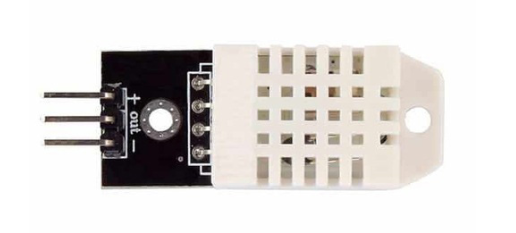
\includegraphics[width=0.4\textwidth]{assets/metodos_herramientas/dht22.png}
    \caption{Sensor DHT22.}
    \label{fig:dht22}
\end{figure}
\begin{itemize}
    \item VCC a 3.3--6 V.
    \item OUT a un pin digital con protocolo 1-wire.
    \item GND a tierra.
\end{itemize}

\begin{figure}[!ht]
    \centering
    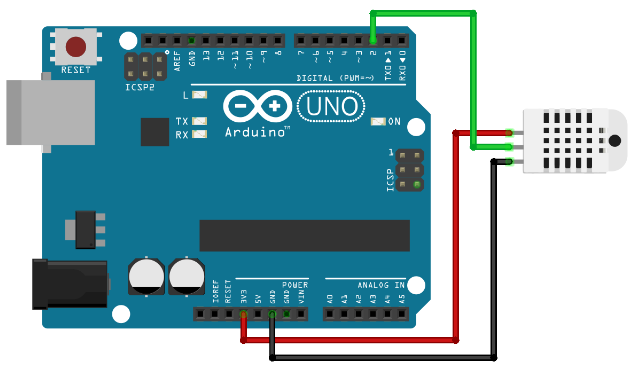
\includegraphics[width=0.5\textwidth]{assets/metodos_herramientas/arduino_dht22.png}
    \caption{Conexión del sensor DHT22 a Arduino.}
    \label{fig:arduino_dht22}
\end{figure}

\paragraph{Herramientas de software}
\begin{itemize}
    \item Arduino IDE 2.2.1 en Windows 10.
    \item Librerías de Adafruit: \texttt{DHT sensor library} y \texttt{Adafruit Unified Sensor}.
\end{itemize}

\subsection{Celda de carga y módulo HX711}
Las celdas de carga son los sensores que recolectan información sobre el peso de una carga aplicada sobre los mismos. Los sensores a utilizar son equivalentes a los de la ilustración 3, cuentan con 4 cables y 4 orificios roscados para fijar la celda, así como una imagen indicativa de la dirección de la carga.

\begin{figure}[!ht]
    \centering
    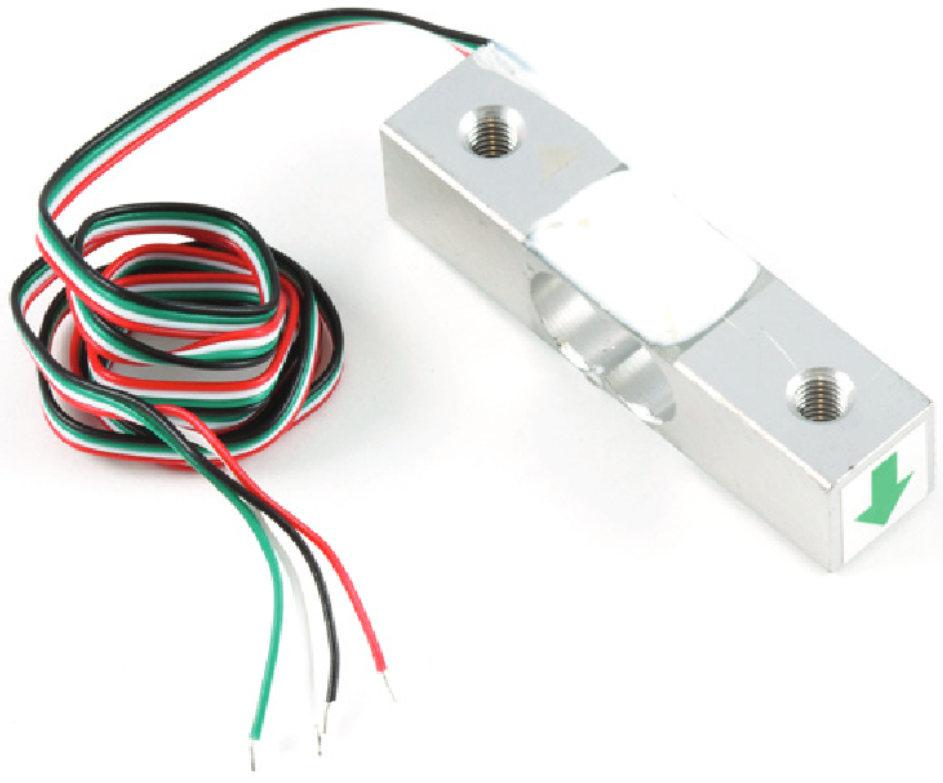
\includegraphics[width=0.5\textwidth]{assets/metodos_herramientas/celda_carga.png}
    \caption{Celda de carga.}
    \label{fig:celda_carga}
\end{figure}
\newpage

El módulo HX711 es una placa electrónica que funciona como interfaz entre una placa Arduino y una celda de carga. Este se muestra en la ilustración \ref{fig:hx711}. El módulo HX711 es un convertidor analógico a digital (ADC) de 24 bits, diseñado específicamente para aplicaciones de pesaje y medición de fuerza. Permite leer las señales analógicas de la celda de carga y convertirlas en valores digitales que pueden ser procesados por un microcontrolador como Arduino.

\begin{figure}[!ht]
    \centering
    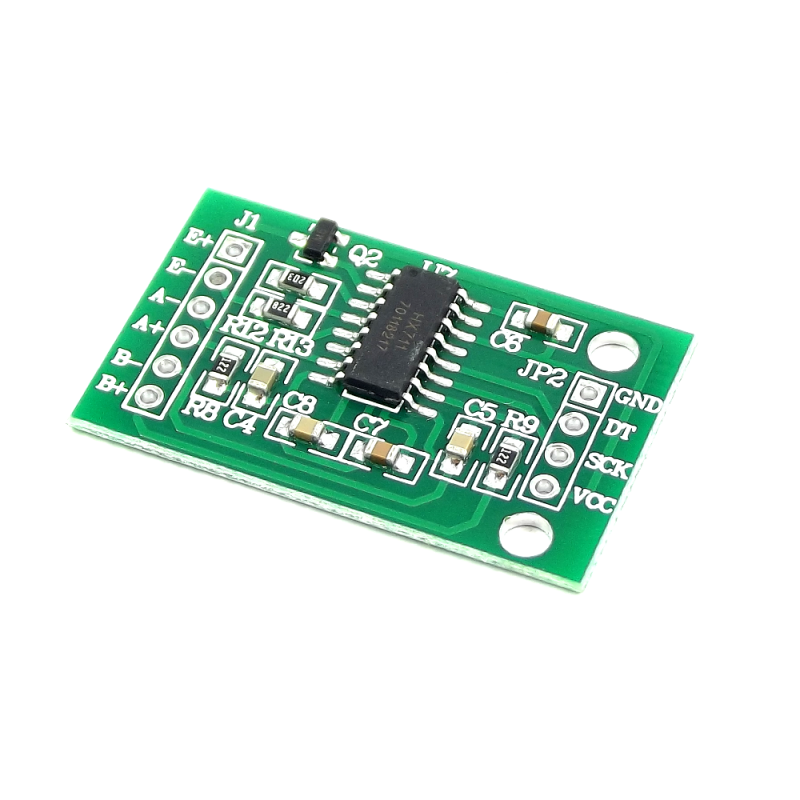
\includegraphics[width=0.5\textwidth]{assets/metodos_herramientas/hx711.png}
    \caption{Módulo HX711.}
    \label{fig:hx711}
\end{figure}
Las conexiones se realizan de acuerdo a las tablas \ref{tab:conexiones_celda_hx711} y \ref{tab:conexiones_hx711_arduino}. La celda de carga se conecta al módulo HX711, y este último se conecta a la placa Arduino. El módulo HX711 requiere una alimentación de 5 V y tiene dos pines de salida: uno para la señal de datos (DT) y otro para el reloj (SCK).
\begin{table}[!ht]
    \centering
    \rowcolors{2}{gray!10}{white}
    \begin{tabularx}{\textwidth}{>{\bfseries}X X}
        \toprule
        \textbf{COLOR DEL CABLE} & \textbf{CONECCIÓN EN MÓDULO} \\
        \midrule
        ROJO                     & E+                           \\
        NEGRO                    & E-                           \\
        BLANCO                   & A-                           \\
        VERDE                    & A+                           \\
        \bottomrule
    \end{tabularx}
    \caption{\textit{conexiones celda-HX711}}
\end{table}
\begin{table}[!ht]
    \centering
    \rowcolors{2}{gray!10}{white}
    \begin{tabularx}{\textwidth}{>{\bfseries}X X}
        \toprule
        \textbf{PIN HX711} & \textbf{CONECCIÓN EN ARDUINO} \\
        \midrule
        GND                & GND                           \\
        DT                 & A1                            \\
        SCK                & A0                            \\
        VCC                & 5 V                           \\
        \bottomrule
    \end{tabularx}
    \caption{\textit{conexiones HX711-Arduino}}
\end{table}
\newpage

\paragraph{Ejemplo de código HX711}\mbox{}

\begin{lstlisting}[language=C++, caption={Ejemplo de código HX711}, label={lst:ejemplo_hx711}]
#include "HX711.h"
const int DOUT = A1;
const int CLK = A0;
HX711 balanza;

void setup() {
  Serial.begin(9600);
  balanza.begin(DOUT, CLK);
  balanza.set_scale(439430.25);
  balanza.tare();
}

void loop() {
  Serial.println(balanza.get_units());
  delay(1000);
}
\end{lstlisting}

\subsection{Controlador ESP32}
El ESP32 integra Wi-Fi y Bluetooth en un solo chip con bajo consumo en modo Deep Sleep (~10 \textmu{}A a 3.3 V).
\begin{itemize}
    \item Procesador: Xtensa LX6, 32 bits, hasta 240 MHz.
    \item RAM: 520 KB SRAM.
\end{itemize}

Para utilizar el controlador con el Arduino IDE2.0 es necesario agregar el siguiente paquete a Additional Boards Manager como se muestra en la figura  \ref{fig:arduino_placas} y el código \ref{lst:esp32_boards_manager}.
\begin{lstlisting}[language=, label={lst:esp32_boards_manager}, caption={URL para Boards Manager de ESP32}]
https://raw.githubusercontent.com/espressif/arduino-esp32/gh-pages/package_esp32_index.json
\end{lstlisting}

\newpage

\begin{figure}[!ht]
    \centering
    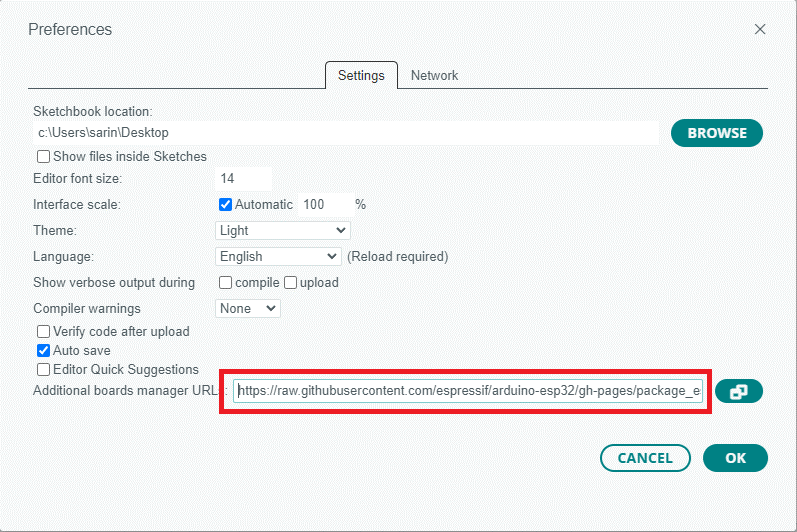
\includegraphics[width=0.75\textwidth]{assets/metodos_herramientas/arduino_placas.png}
    \caption{Selección de placas ESP32 en Arduino IDE.}
    \label{fig:arduino_placas}
\end{figure}

El siguiente paso es instalar los controladores para la placa ESP32, se muestra en la figura  \ref{fig:arduino_install_esp32}.

\begin{figure}[!ht]
    \centering
    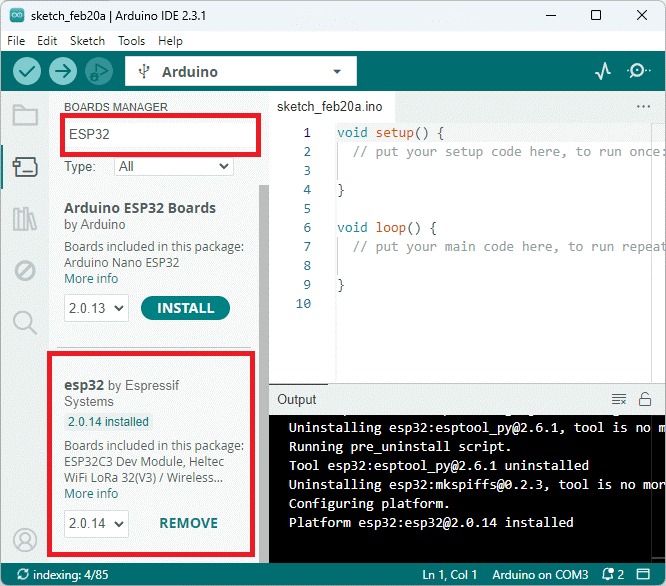
\includegraphics[width=0.75\textwidth]{assets/metodos_herramientas/arduino_install_esp32.png}
    \caption{Instalación del soporte para ESP32 en Arduino IDE.}
    \label{fig:arduino_install_esp32}
\end{figure}

\newpage

Código de prueba:
\begin{lstlisting}[language=C++, label={lst:esp32_blink}, caption={Ejemplo de código de parpadeo de LED en ESP32}]
#include <Arduino.h>
#define LED 2
void setup() {
  Serial.begin(115200);
  pinMode(LED, OUTPUT);
}
void loop() {
  digitalWrite(LED, HIGH);
  delay(1000);
  digitalWrite(LED, LOW);
  delay(1000);
}
\end{lstlisting}

\subsection{Micrófono INMP441}
\begin{figure}[!ht]
    \centering
    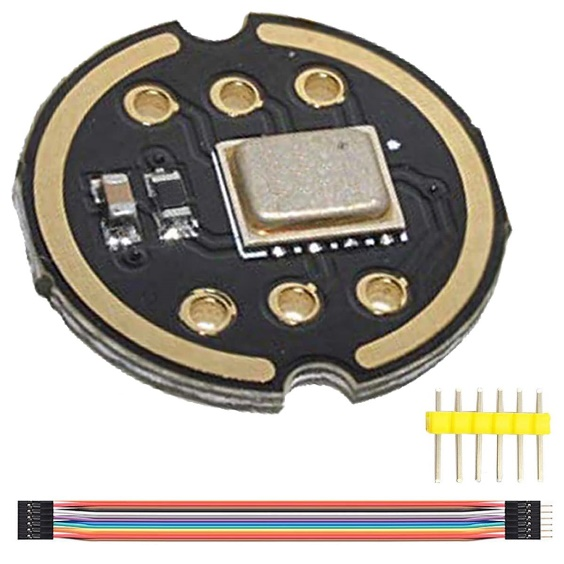
\includegraphics[width=0.75\textwidth]{assets/metodos_herramientas/inmp441.png}
    \caption{Módulo de micrófono INMP441.}
    \label{fig:inmp441}
\end{figure}

El sensor INMP441 es un micrófono multidireccional que utiliza el protocolo I2S~\cite{keysight_i2s_blog} para transferencia de audio, de la misma manera que, y como se mencionó en los trabajos relacionados, el dispositivo INMP401 es utilizado con el controlador ESP8266, el dispositivo INMP441 es comúnmente utilizado con el dispositivo ESP32, principalmente por su compatibilidad mediante el protocolo I2S. El módulo INMP441 se muestra en la figura  7~\cite{inmp441_datasheet}.


\chapter{Estado del arte}
\label{chap:estado_arte}

\section{Marco teórico}
\subsection{Introducción}
La implementación de la infraestructura de telecomunicaciones ha transformado numerosos aspectos de la vida cotidiana y el ámbito industrial, dando lugar a innovaciones que facilitan la comunicación y el control de diversos sistemas. Uno de estos avances es el Internet de las Cosas (IoT), que conecta objetos físicos a la red, permitiendo su monitoreo y control a través de dispositivos electrónicos y software. En este contexto, en el área de la apicultura se han adoptado tecnologías IoT para mejorar la gestión y el monitoreo de las colmenas, creando lo que se conoce como colmenas inteligentes.

En este capítulo se ofrece un marco teórico sobre los conceptos clave del internet, IoT y su aplicación en la apicultura. Se explora la arquitectura IoT, desglosada en sus siete capas fundamentales, y se examina la interacción de los sensores en estos sistemas. Además, se profundiza en el uso de IoT en las colmenas, destacando su capacidad para monitorear parámetros críticos como la temperatura, la humedad y el peso de la colmena, así como para detectar el enjambrado a través del análisis de sonidos específicos. También se proporciona una visión general sobre la inteligencia artificial y su potencial integración en sistemas IoT para optimizar el control y análisis de datos en la apicultura.
\subsection{Apicultura}
Se refiere a la crianza y explotación de abejas, de las cuales se obtienen productos como miel, cera y polen, y que al mismo tiempo realizan el servicio de polinización de plantas.

\subsection{Abejas}
Se refiere a un insecto social que durante su ciclo de vida se encarga de producir miel, cera y panal y polinizar plantas para apoyarlas en su reproducción, por lo cual se les considera de los insectos más importantes del planeta.  \cite{david_cramp}

\subsection{Colmena}
Una abeja no puede sobrevivir de manera individual, una abeja obrera no se puede reproducir y una abeja reina no puede construir o mantener una colmena ya que la estructura social de las abejas requiere de a las obreras, las reinas y los drones para sobrevivir, por lo cual se considera a la misma como un organismo independiente. \cite{david_cramp} En la figura~\ref{fig:abejas} se muestra una imagen ilustrativa de las 3 castas de abeja.

\begin{figure}[htbp]
  \centering
  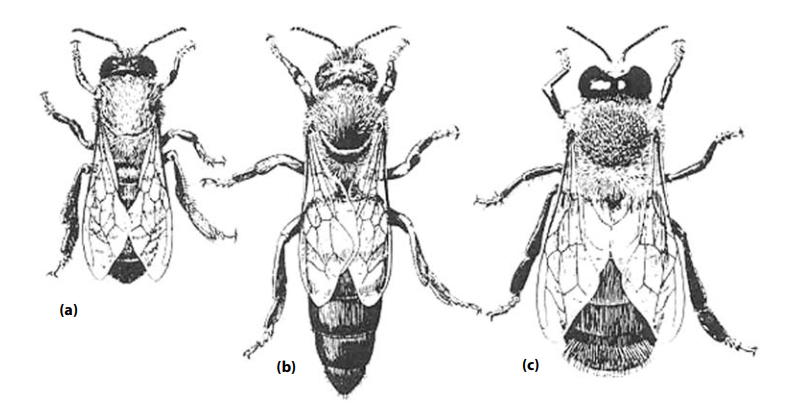
\includegraphics[width=0.75\textwidth]{assets/abejas.png}
  \caption{Castas de abejas. \cite{david_cramp}}
  \label{fig:abejas}
\end{figure}

Como se observa en la figura~\ref{fig:abejas}, las castas de abejas son las siguientes:
\begin{enumerate}
  \renewcommand\labelenumi{\alph{enumi})}
  \item \textbf{Obreras}: Estas se encargan de todas las tareas no relacionadas con la reproducción, incluyendo la construcción del panal, la recolección de polen, la producción de miel, entre otras actividades vitales para la colmena.
  \item \textbf{Reinas}: Son la única hembra completa de la colonia; su única responsabilidad es reproducirse y poner huevos.
  \item \textbf{Drones}: Similar a la reina; su única responsabilidad es reproducirse con reinas de otras colonias.
\end{enumerate}

\subsection{Temperatura de la colmena}
Una colmena debe de mantener una temperatura cercana a los 34 grados centígrados, para lograr esto pueden implementar ciertos mecanismos de regulación de temperatura. \cite{david_cramp}
Cuando las abejas necesitan elevar la temperatura, generan una capa de abejas vivas alrededor de la reina, después proceden a vibrar con el objetivo de producir calor. Para este proceso es necesario que la colmena cuente con suficiente alimento, además, se apoya del aislamiento de la colmena, ya sea natural o artificial, de modo natural, la miel y la cera son buenos aislantes. \cite{chadwick_alton_tennant_fitzmaurice_earl_2016}
Por otro lado, las abejas suelen iniciar un aleteo con sus alas para reducir la temperatura dentro de la colmena. \cite{chadwick_alton_tennant_fitzmaurice_earl_2016}

\subsection{Humedad de la colmena}
La humedad tiene un papel importante en la prevención de enfermedades dentro de la colmena, por esta razón es de importancia para las abejas controlar esta propiedad, el mecanismo que utilizan las abejas en estos casos es utilizar sus alas como ventiladores para expulsar la humedad de la colmena. \cite{chadwick_alton_tennant_fitzmaurice_earl_2016}

\subsection{Peso de la colmena}
El peso es el principal factor utilizado por los apicultores para medir la cantidad en los almacenes de miel, de manera tradicional, los apicultores intentan levantar la colmena, en caso de no ser capaces, consideran que la miel esta lista para ser extraída \cite{chadwick_alton_tennant_fitzmaurice_earl_2016}, de manera precisa, se considera una extracción cuando el almacén de miel pesa cerca a los 40kg.\cite{david_cramp}

\subsection{Enjambrado}
El evento de enjambre sucede cuando una colonia de abejas ha sobrepasado el límite físico de la colmena en la que habita, este proceso comienza con la reina engendrando nuevas reinas y drones, después de esto un enjambre de abejas y drones emigran a un nuevo posible lugar en el cual comienza una nueva colmena. \cite{chadwick_alton_tennant_fitzmaurice_earl_2016}

Uno de los principales indicadores del enjambrado es el sonido que emiten las abejas, durante este proceso comienzan a emitir un sonido de vibración, este sonido es conocido por los apicultores y es la principal fuente de información que se obtiene sobre este proceso \cite{david_cramp} \cite{chadwick_alton_tennant_fitzmaurice_earl_2016}.

\subsection{Internet e IoT}

\subsubsection{Internet}
En el contexto actual, internet se refiere a una red global con varios protocolos de conectividad que permite comunicar paquetes de datos de dispositivos, mediante un sistema de rúters, a la red. \cite{kamal_2017}

\subsubsection{Rúter, router o enrutador}
Se refiere a un dispositivo capaz de almacenar direcciones y enlaces mediante las cuales se encarga de mandar paquetes de datos.\cite{kamal_2017}

\subsubsection{Internet de las cosas (IoT)}
El termino de internet de las coas, o IOT por sus siglas en inglés (Internet of things), se refiere al concepto de entrelazar objetos físicos dentro de una red de internet, mediante componentes electrónicos y sistemas de software, con el objetivo de permitir la comunicación entre ellos y monitorear o controlar un sistema físico. \cite{kamal_2017}

\subsubsection{Arquitectura IoT}
Este concepto se refiere a la forma de estructurar u diseñar un sistema IOT y estos se dividen en capas y son 7 principales
\begin{enumerate}
  \renewcommand\labelenumi{\arabic{enumi}.}
  \item Componentes físicos: sensores y controladores.
  \item Dispositivos de conectividad.
  \item Computación perimetral (análisis de datos y procesamiento).
  \item Persistencia de datos.
  \item Abstracción de datos (acceso y manipulación).
  \item Aplicación (reportes, análisis y control).
  \item Colaboración y procesos (usuarios y procesos comerciales).
\end{enumerate}
Estas capas sirven para estructurar y definir la arquitectura del sistema IOT.\cite{kamal_2017}


\subsubsection{Sensores}
El sistema IOT interactúa con sensores, dispositivos físicos con el objetivo de adquirir datos mediante la capacidad de reaccionar a parámetros físicos como la humedad, temperatura, presión y luz y convertirla en energía eléctrica capaz de interactuar con el sistema. Durante esta interacción es posible configurar los dispositivos de manera que se ajusten a los requerimientos de la aplicación.\cite{kamal_2017}

\subsubsection{Colmenas inteligentes}
Los términos Colmenas IOT o colmenas inteligentes se refieren a la adición de un sistema IOT a una colmena apícola, esto con el objetivo de monitorear los parámetros de la colonia de abejas y hacer accesible la información de manera que pueda ser procesada para conocer el estado de la colmena. \cite{open_source_beehives_project_iaac}

\subsection{Inteligencia artificial}

\subsubsection{Sistema inteligente}
Se refiere a un concepto abstracto en el cual se define a un sistema que actúa y razona de manera humana o de manera lógica \cite{russell_norvig_2022}. Es uno de los posibles métodos para procesar datos de un sistema IOT \cite{open_source_beehives_project_iaac}.

\subsubsection{Minería de datos}
Se refiere al proceso de aplicar métodos computacionales a grandes cantidades de datos con el objetivo de revelar información nueva, no trivial y relevante \cite{fayyad1996kdd}. Esto incluye la aplicación de algoritmos específicos para la extracción de patrones, la limpieza de datos, el preprocesamiento y la extracción de características.


\subsubsection{Preprocesamiento de datos}
El preprocesamiento de datos es una etapa en la minería de datos que consiste en preparar y limpiar el conjunto de datos con el objetivo de mejorar su calidad para que sean adecuados para el análisis o modelado. Esto implica corregir valores inválidos, eliminar columnas irrelevantes, manejar valores faltantes, ajustar datos inconsistentes, entre otros \cite{statistical_modeling_in_machine_learning_2023}.

\subsubsection{Aprendizaje automático}
El aprendizaje automático, o aprendizaje maquina, es una rama de la inteligencia artificial que se centra en desarrollar algoritmos capaces de aprender automáticamente a partir de los datos y mejorar su desempeño con la experiencia, sin ser programados explícitamente. Formalmente, se dice que un programa aprende de una experiencia $E$ respecto a una clase de tareas $T$ y una medida de desempeño $P$, si su desempeño en las tareas de $T$, medida por $P$, mejora con la experiencia $E$. En otras palabras, el desempeño del algoritmo en una tarea mejora conforme gana experiencia al realizarla \cite{mitchell1997machine}.


\subsubsection{Extracción de características}
La extracción de características es una técnica de preprocesamiento de datos utilizada en el aprendizaje máquina para transformar un conjunto de datos complejos y con muchas características, en un espacio más manejable y representativo. Se utiliza cuando hay demasiadas características ya sea para un análisis efectivo o para la visualización de datos \cite{richer_coelho_2013}.

\subsubsection{Características de audio}

\begin{itemize}
  \item \textbf{Zero Crossing Rate (ZCR):} Número de veces que la señal cruza el eje cero por unidad de tiempo. Indica la frecuencia de cambios en la señal, útil para distinguir sonidos ruidosos y tonales \cite{muller2015fmp}.

  \item \textbf{RMS (Root Mean Square):} Raíz cuadrada del promedio cuadrático de las muestras; mide energía promedio de la señal, útil para comparar su intensidad relativa entre segmentos \cite{sound_quality_heyboer2010}.

  \item \textbf{Energía:} Suma de los cuadrados de las amplitudes de la señal, representa la potencia o intensidad del sonido \cite{rabiner2010fundamentals}.

  \item \textbf{Entropía de energía:} Mide la distribución y variabilidad de la energía dentro de una señal, calculada usando entropía de Shannon sobre segmentos de energía \cite{li2017audio}.

  \item \textbf{Centroide espectral:} Promedio ponderado de las frecuencias presentes en una señal, que refleja el "brillo" percibido del sonido \cite{peeters2004large}.

  \item \textbf{Dispersión espectral:} Desviación estándar de la distribución espectral alrededor del centroide, indica la extensión del contenido frecuencial \cite{peeters2004large}.

  \item \textbf{Entropía espectral:} Entropía de Shannon aplicada a la densidad espectral de potencia, mide la complejidad del espectro \cite{jiang2011spectral}.

  \item \textbf{Flujo espectral:} Cambio en el espectro de potencia entre frames consecutivos, usado para detectar transiciones y dinámica en la señal \cite{foote2000novelty}.

  \item \textbf{Rolloff espectral:} Frecuencia debajo de la cual se acumula un porcentaje dado (e.g., 85\%) de la energía espectral, útil para distinguir sonidos agudos de graves \cite{tzanetakis2002musical}.

  \item \textbf{MFCC (1 a 13):} Coeficientes cepstrales calculados sobre la escala de frecuencias Mel, que modelan el timbre y la estructura espectral, ampliamente usados en reconocimiento de voz y análisis musical \cite{davis1980tassp}.
\end{itemize}




\section{Trabajos relacionados}
La adición de tecnologías de internet de las cosas (IoT) en la apicultura ha significado un cambio revolucionario a comparación de las prácticas tradicionales, aumentando la eficiencia, productividad y escalabilidad. Estas tecnologías involucran el uso de diferentes sistemas interconectados, incluyendo sensores, microcontroladores y software, con el objetivo de ayudar a monitorear y administrar las actividades apícolas en tiempo real.
En este capítulo se exploran las aplicaciones relevantes en las cuales se han desarrollado las aplicaciones de IoT en el monitoreo de colmenas apícolas, con el objetivo de dar seguimiento a la salud y actividad de las colonias de abejas, proveyendo así información de la colmena, incluyendo parámetros como temperatura, humedad, peso y acústica que ayudan a los apicultores a mantener colonias saludables y tomar decisiones acordes a la información en tiempo real.
La arquitectura de sistemas IoT para monitoreo de colmenas involucra varios componentes clave, incluyendo nodos de sensores, sistemas de transmisión de datos, sistemas de energía y el componente de procesamiento de datos. En este capítulo se examinan las prácticas utilizadas para implementar estos sistemas.

\subsection{Embedded Software for IoT Bee Hive Monitoring Node}
Este artículo presenta un sistema embebido para monitoreo de variables relevantes; se propone un sistema que tiene las capacidades de monitorear humedad, temperatura, peso y audio. Sin embargo, solo se detalla la implementación del monitoreo de humedad y temperatura. Para este sistema se utilizó el sensor SHT21~\cite{sht21} para la medición de temperatura y humedad.~\cite{vidrascu_svasta_2017a}  
El sistema está construido alrededor del componente ESP8266 que integra un microcontrolador Tensilica L106 de 32 bits en conjunto con el módulo transmisor Wi-Fi que integra circuitos de radiofrecuencia y es capaz de transmitir datos mediante interfaces digitales como SPI, I2C, y UART. Además, el módulo ESP8266 cuenta con tres modos de operación: activo, dormido y dormido profundo, los cuales son aprovechados por el sistema para optimizar el uso de energía.~\cite{vidrascu_svasta_2017a}

\subsection{A Smart Sensor-Based Measurement System for Advanced Bee Hive Monitoring}
Este sistema desarrolla un monitoreo de parámetros relevantes para la colmena, incluyendo peso, sonido, temperatura, humedad y CO$_2$.~\cite{cecchi_spinsante_terenzi_orcioni_2020}  
Es modular y se compone de dos módulos principales:  
\begin{itemize}
    \item \textbf{Módulo Abeja}: Raspberry Pi 3B~\cite{buy_raspberry_pi3_model_b}, tarjeta de sonido UCA22~\cite{behringer_uca222}, micrófonos ADMP401 MEMS~\cite{admp401_datasheet}, sensores DHT22~\cite{liu}, células de carga TAL220~\cite{loadcell_tal220_sparkfun} con HX711~\cite{hx711_sparkfun} y sensor de CO$_2$ TL6615~\cite{t6615_telaire}.
    \item \textbf{Módulo Reina}: Raspberry Pi 3B, sensores DHT22 y un puente 5G (no especificado) utilizado para comunicarse con el servidor remoto.~\cite{cecchi_spinsante_terenzi_orcioni_2020}
\end{itemize}  
Este artículo se energiza mediante una conexión a la red eléctrica, los módulos Reina y Abeja consumen 4 y 4.2 watts respectivamente.~\cite{cecchi_spinsante_terenzi_orcioni_2020}

\subsection{High Reliability Wireless Sensor Node for Bee Hive Monitoring}
Este sistema está diseñado para condiciones de entre -20 a 60 °C con una arquitectura modular que permite intercambiar sensores mediante interfaz I2C.~\cite{vidrascu_svasta_vladescu_2016}  
Incluye sensores SHT21, sistema HX711 con células de carga, sensor de inclinación DMA08 y micrófono MP34DT05-A.~\cite{vidrascu_svasta_vladescu_2016}  
Además, utiliza un módulo ESP8266 serie 32-bit a 80MHz para conexión Wi-Fi directa.~\cite{vidrascu_svasta_vladescu_2016}  
En cuanto a la energía, se emplean supercapacitores XV de Eaton~\cite{supercapacitor_xv_eaton} junto con paneles solares (no especificados) y un convertidor step up.~\cite{vidrascu_svasta_vladescu_2016}

\subsection{Bee Swarm Activity Acoustic Classification for an IoT-Based Farm Service}
Este sistema utiliza un micrófono TDK InvenSense ICS-40300 y una placa Atmel ATmega32U4 sobre la colmena, procesando los datos en un servidor remoto.~\cite{zgank_2019}  
El procesamiento de datos acústicos tiene como objetivo la detección de enjambres, utilizando datos del Open Source Beehives Project (OSBP)~\cite{open_source_beehives_project_iaac}. Se aplican métodos MFCC y LPC para extracción de características y HMM/GMM para clasificación.~\cite{zgank_2019}

\subsection{Maintenance-free IoT Gateway Design for Bee Hive Monitoring}
Este módulo recopila información con sensores SHT21, MPL3115A2~\cite{nxp_mpl3115a2}, TSL2561~\cite{tsl2561_adafruit}, HX711, VEML6075~\cite{adafruit_veml6075} y GP2Y1010AU0F~\cite{vidrascu_svasta_2017b}.~\cite{vidrascu_svasta_2017b}  
Para transmisión de datos se utiliza un ESP8266-12 (A.I.Thinker) y un módem A6 GSM/GPRS (no en bib).~\cite{vidrascu_svasta_2017b}  
El sistema obtiene energía de paneles solares (no especificados) con reguladores LT3652~\cite{lt3652_datasheet} y LTC3652~\cite{ltc3652_datasheet}.~\cite{vidrascu_svasta_2017b}

\subsection{A Pi-Based IoT System Design}
Este sistema integra la suite de sensores GrovePi: humedad, temperatura, GPS, sonido e imágenes térmicas.~\cite{chen_chien_hsu_jing_lin_lin_2020}  
Implementa múltiples módulos Wi-Fi conectados a un módem independiente con conexión a red móvil.~\cite{chen_chien_hsu_jing_lin_lin_2020}  
Se alimenta con una batería de 10000 mAh (180000 J a 5V), con autonomía de 27–33 h.~\cite{chen_chien_hsu_jing_lin_lin_2020}

\subsection{Conclusión}
A lo largo de este capítulo, se han explorado diversas arquitecturas y tecnologías utilizadas en estos sistemas, destacando los componentes esenciales como los nodos de sensores y los sistemas de transmisión de datos, así como las soluciones innovadoras para el manejo de energía y el procesamiento de datos.
\begin{itemize}
    \item \textbf{Nodos de Sensores}: Los sistemas presentados varían en complejidad, pero todos incluyen sensores de temperatura, humedad, peso y acústica.
    \item \textbf{Sistemas de Transmisión de Datos}: Predomina el uso del módulo ESP8266, con casos que incorporan GSM/GPRS.
    \item \textbf{Manejo de Energía}: Paneles solares, baterías y supercapacitores son las soluciones más comunes.
    \item \textbf{Procesamiento de Datos}: Se emplean MFCC, LPC, HMM y GMM en clasificación de eventos acústicos.
\end{itemize}
La adición de tecnologías de internet de las cosas (IoT) en la apicultura ha significado un cambio revolucionario a comparación de las prácticas tradicionales, aumentando la eficiencia, productividad y escalabilidad. Estas tecnologías involucran el uso de diferentes sistemas interconectados, incluyendo sensores, microcontroladores y software, con el objetivo de ayudar a monitorear y administrar las actividades apícolas en tiempo real.
En este capítulo se exploran las aplicaciones relevantes en las cuales se han desarrollado las aplicaciones de IoT en el monitoreo de colmenas apícolas, con el objetivo de dar seguimiento a la salud y actividad de las colonias de abejas, proveyendo así información de la colmena, incluyendo parámetros como temperatura, humedad, peso y acústica que ayudan a los apicultores a mantener colonias saludables y tomar decisiones acordes a la información en tiempo real.
La arquitectura de sistemas IoT para monitoreo de colmenas involucra varios componentes clave, incluyendo nodos de sensores, sistemas de transmisión de datos, sistemas de energía y el componente de procesamiento de datos. En este capítulo se examinan las prácticas utilizadas para implementar estos sistemas.

\subsection{Embedded Software for IoT Bee Hive Monitoring Node}
Este artículo presenta un sistema embebido para monitoreo de variables relevantes; se propone un sistema que tiene las capacidades de monitorear humedad, temperatura, peso y audio. Sin embargo, no se implementó el monitoreo de peso y audio. Para este sistema se utilizó el sensor SHT21~\cite{sht21} para la medición de temperatura y humedad.~\cite{vidrascu_svasta_2017a}  
El sistema está construido alrededor del componente ESP8266 que integra un microcontrolador Tensilica L106 32-bit en conjunto con el módulo transmisor Wi-Fi que integra circuitos de radio frecuencia y es capaz de transmitir datos mediante interfaces digitales como SPI, I2C, y UART. Además, el módulo ESP8266 cuenta con tres modos de operación: activo, dormido y dormido profundo, los cuales son aprovechados por el sistema para optimizar el uso de energía.~\cite{vidrascu_svasta_2017a}

\subsection{A Smart Sensor-Based Measurement System for Advanced Bee Hive Monitoring}
Este sistema desarrolla un monitoreo de parámetros relevantes para la colmena, incluyendo peso, sonido, temperatura, humedad y CO$_2$.~\cite{cecchi_spinsante_terenzi_orcioni_2020}  
Es modular y se compone de dos módulos principales:  
\begin{itemize}
    \item \textbf{Módulo Abeja}: Raspberry Pi 3B~\cite{buy_raspberry_pi3_model_b}, tarjeta de sonido UCA22~\cite{behringer_uca222}, micrófonos ADMP401 MEMS~\cite{admp401_datasheet}, sensores DHT22~\cite{liu}, células de carga TAL220~\cite{loadcell_tal220_sparkfun} con HX711~\cite{hx711_sparkfun} y sensor de CO$_2$ TL6615~\cite{t6615_telaire}.
    \item \textbf{Módulo Reina}: Raspberry Pi 3B, sensores DHT22 y un puente 5G (no especificado) utilizado para comunicarse con el servidor remoto.~\cite{cecchi_spinsante_terenzi_orcioni_2020}
\end{itemize}  
Este artículo se energiza mediante una conexión a la red eléctrica, los módulos Reina y Abeja consumen 4 y 4.2 watts respectivamente.~\cite{cecchi_spinsante_terenzi_orcioni_2020}

\subsection{High Reliability Wireless Sensor Node for Bee Hive Monitoring}
Este sistema está diseñado para condiciones de entre -20 a 60 °C con una arquitectura modular que permite intercambiar sensores mediante interfaz I2C.~\cite{vidrascu_svasta_vladescu_2016}  
Incluye sensores SHT21, sistema HX711 con células de carga, sensor de inclinación DMA08 y micrófono MP34DT05-A.~\cite{vidrascu_svasta_vladescu_2016}  
Además, utiliza un módulo ESP8266 serie 32-bit a 80MHz para conexión Wi-Fi directa.~\cite{vidrascu_svasta_vladescu_2016}  
En cuanto a la energía, se emplean supercapacitores XV de Eaton~\cite{supercapacitor_xv_eaton} junto con paneles solares (no especificados) y un convertidor step up.~\cite{vidrascu_svasta_vladescu_2016}

\subsection{Bee Swarm Activity Acoustic Classification for an IoT-Based Farm Service}
Este sistema utiliza un micrófono TDK InvenSense ICS-40300 y una placa Atmel ATmega32U4 sobre la colmena, procesando los datos en un servidor remoto.~\cite{zgank_2019}  
El procesamiento de datos acústicos tiene como objetivo la detección de enjambres, utilizando datos del Open Source Beehives Project (OSBP)~\cite{open_source_beehives_project_iaac}. Se aplican métodos MFCC y LPC para extracción de características y HMM/GMM para clasificación.~\cite{zgank_2019}

\subsection{Maintenance-free IoT Gateway Design for Bee Hive Monitoring}
Este módulo recopila información con sensores SHT21, MPL3115A2~\cite{nxp_mpl3115a2}, TSL2561~\cite{tsl2561_adafruit}, HX711, VEML6075~\cite{adafruit_veml6075} y GP2Y1010AU0F~\cite{vidrascu_svasta_2017b}.~\cite{vidrascu_svasta_2017b}  
Para transmisión de datos se utiliza un ESP8266-12 (A.I.Thinker) y un módem A6 GSM/GPRS (no en bib).~\cite{vidrascu_svasta_2017b}  
El sistema obtiene energía de paneles solares (no especificados) con reguladores LT3652~\cite{lt3652_datasheet} y LTC3652~\cite{ltc3652_datasheet}.~\cite{vidrascu_svasta_2017b}

\subsection{A Pi-Based IoT System Design}
Este sistema integra la suite de sensores GrovePi: humedad, temperatura, GPS, sonido e imágenes térmicas.~\cite{chen_chien_hsu_jing_lin_lin_2020}  
Implementa múltiples módulos Wi-Fi conectados a un módem independiente con conexión a red móvil.~\cite{chen_chien_hsu_jing_lin_lin_2020}  
Se alimenta con una batería de 10000 mAh (180000 J a 5V), con autonomía de 27–33 h.~\cite{chen_chien_hsu_jing_lin_lin_2020}

\subsection{Conclusión}
A lo largo de este capítulo, se han explorado diversas arquitecturas y tecnologías utilizadas en estos sistemas, destacando los componentes esenciales como los nodos de sensores y los sistemas de transmisión de datos, así como las soluciones innovadoras para el manejo de energía y el procesamiento de datos.
\begin{itemize}
    \item \textbf{Nodos de Sensores}: Los sistemas presentados varían en complejidad, pero todos incluyen sensores de temperatura, humedad, peso y acústica.
    \item \textbf{Sistemas de Transmisión de Datos}: Predomina el uso del módulo ESP8266, con casos que incorporan GSM/GPRS.
    \item \textbf{Manejo de Energía}: Paneles solares, baterías y supercapacitores son las soluciones más comunes.
    \item \textbf{Procesamiento de Datos}: Se emplean MFCC, LPC, HMM y GMM en clasificación de eventos acústicos.
\end{itemize}


\section{Métodos y herramientas}
\subsection{Sensor DHT22}

El sensor DHT22 mide temperatura y humedad. Se conecta de la siguiente manera:
\begin{figure}[!ht]
    \centering
    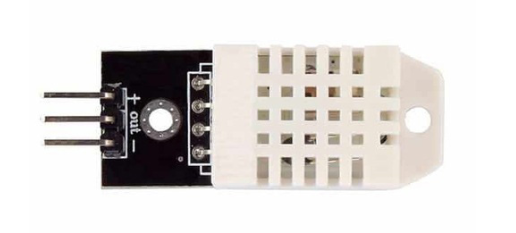
\includegraphics[width=0.4\textwidth]{assets/metodos_herramientas/dht22.png}
    \caption{Sensor DHT22.}
    \label{fig:dht22}
\end{figure}
\begin{itemize}
    \item VCC a 3.3--6 V.
    \item OUT a un pin digital con protocolo 1-wire.
    \item GND a tierra.
\end{itemize}

\begin{figure}[!ht]
    \centering
    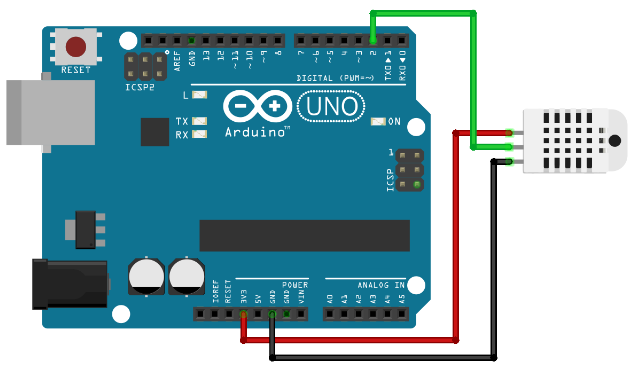
\includegraphics[width=0.5\textwidth]{assets/metodos_herramientas/arduino_dht22.png}
    \caption{Conexión del sensor DHT22 a Arduino.}
    \label{fig:arduino_dht22}
\end{figure}

\paragraph{Herramientas de software}
\begin{itemize}
    \item Arduino IDE 2.2.1 en Windows 10.
    \item Librerías de Adafruit: \texttt{DHT sensor library} y \texttt{Adafruit Unified Sensor}.
\end{itemize}

\subsection{Celda de carga y módulo HX711}
Las celdas de carga son los sensores que recolectan información sobre el peso de una carga aplicada sobre los mismos. Los sensores a utilizar son equivalentes a los de la ilustración 3, cuentan con 4 cables y 4 orificios roscados para fijar la celda, así como una imagen indicativa de la dirección de la carga.

\begin{figure}[!ht]
    \centering
    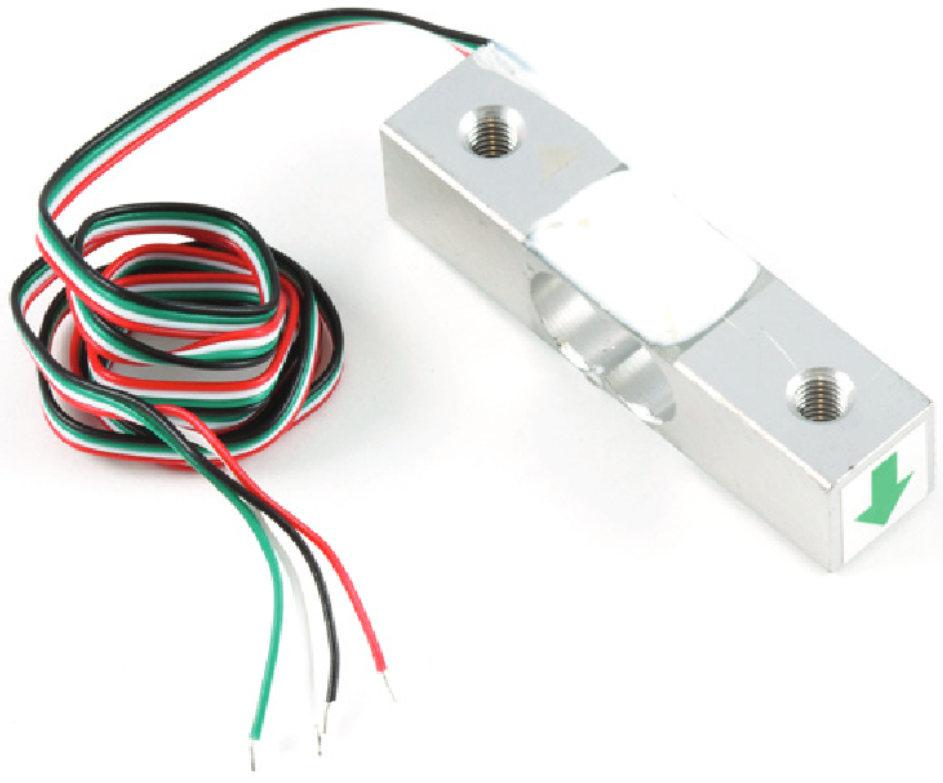
\includegraphics[width=0.5\textwidth]{assets/metodos_herramientas/celda_carga.png}
    \caption{Celda de carga.}
    \label{fig:celda_carga}
\end{figure}
\newpage

El módulo HX711 es una placa electrónica que funciona como interfaz entre una placa Arduino y una celda de carga. Este se muestra en la ilustración \ref{fig:hx711}. El módulo HX711 es un convertidor analógico a digital (ADC) de 24 bits, diseñado específicamente para aplicaciones de pesaje y medición de fuerza. Permite leer las señales analógicas de la celda de carga y convertirlas en valores digitales que pueden ser procesados por un microcontrolador como Arduino.

\begin{figure}[!ht]
    \centering
    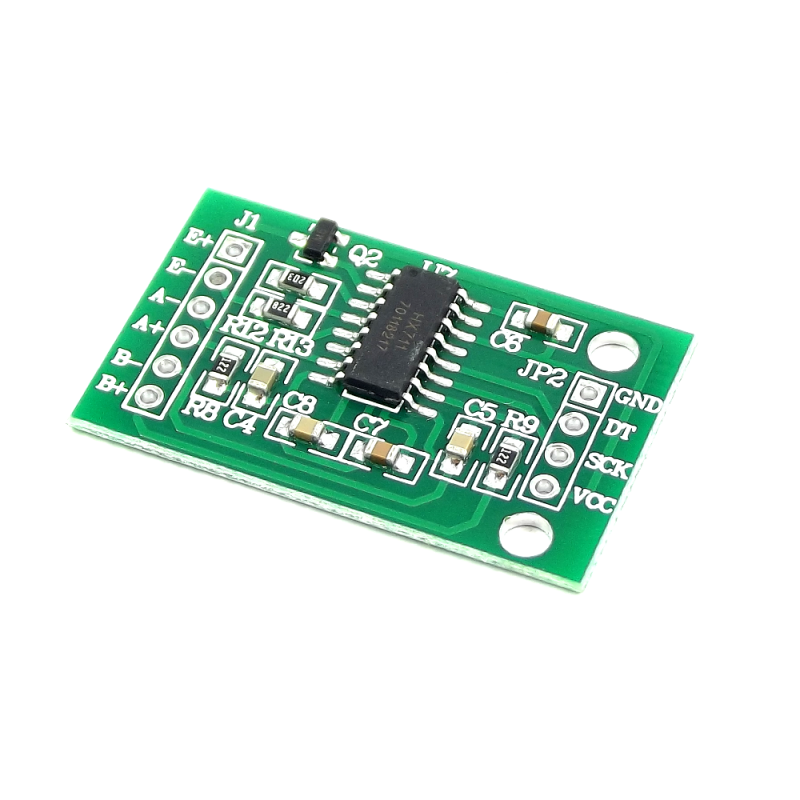
\includegraphics[width=0.5\textwidth]{assets/metodos_herramientas/hx711.png}
    \caption{Módulo HX711.}
    \label{fig:hx711}
\end{figure}
Las conexiones se realizan de acuerdo a las tablas \ref{tab:conexiones_celda_hx711} y \ref{tab:conexiones_hx711_arduino}. La celda de carga se conecta al módulo HX711, y este último se conecta a la placa Arduino. El módulo HX711 requiere una alimentación de 5 V y tiene dos pines de salida: uno para la señal de datos (DT) y otro para el reloj (SCK).
\begin{table}[!ht]
    \centering
    \rowcolors{2}{gray!10}{white}
    \begin{tabularx}{\textwidth}{>{\bfseries}X X}
        \toprule
        \textbf{COLOR DEL CABLE} & \textbf{CONECCIÓN EN MÓDULO} \\
        \midrule
        ROJO                     & E+                           \\
        NEGRO                    & E-                           \\
        BLANCO                   & A-                           \\
        VERDE                    & A+                           \\
        \bottomrule
    \end{tabularx}
    \caption{\textit{conexiones celda-HX711}}
\end{table}
\begin{table}[!ht]
    \centering
    \rowcolors{2}{gray!10}{white}
    \begin{tabularx}{\textwidth}{>{\bfseries}X X}
        \toprule
        \textbf{PIN HX711} & \textbf{CONECCIÓN EN ARDUINO} \\
        \midrule
        GND                & GND                           \\
        DT                 & A1                            \\
        SCK                & A0                            \\
        VCC                & 5 V                           \\
        \bottomrule
    \end{tabularx}
    \caption{\textit{conexiones HX711-Arduino}}
\end{table}
\newpage

\paragraph{Ejemplo de código HX711}\mbox{}

\begin{lstlisting}[language=C++, caption={Ejemplo de código HX711}, label={lst:ejemplo_hx711}]
#include "HX711.h"
const int DOUT = A1;
const int CLK = A0;
HX711 balanza;

void setup() {
  Serial.begin(9600);
  balanza.begin(DOUT, CLK);
  balanza.set_scale(439430.25);
  balanza.tare();
}

void loop() {
  Serial.println(balanza.get_units());
  delay(1000);
}
\end{lstlisting}

\subsection{Controlador ESP32}
El ESP32 integra Wi-Fi y Bluetooth en un solo chip con bajo consumo en modo Deep Sleep (~10 \textmu{}A a 3.3 V).
\begin{itemize}
    \item Procesador: Xtensa LX6, 32 bits, hasta 240 MHz.
    \item RAM: 520 KB SRAM.
\end{itemize}

Para utilizar el controlador con el Arduino IDE2.0 es necesario agregar el siguiente paquete a Additional Boards Manager como se muestra en la figura  \ref{fig:arduino_placas} y el código \ref{lst:esp32_boards_manager}.
\begin{lstlisting}[language=, label={lst:esp32_boards_manager}, caption={URL para Boards Manager de ESP32}]
https://raw.githubusercontent.com/espressif/arduino-esp32/gh-pages/package_esp32_index.json
\end{lstlisting}

\newpage

\begin{figure}[!ht]
    \centering
    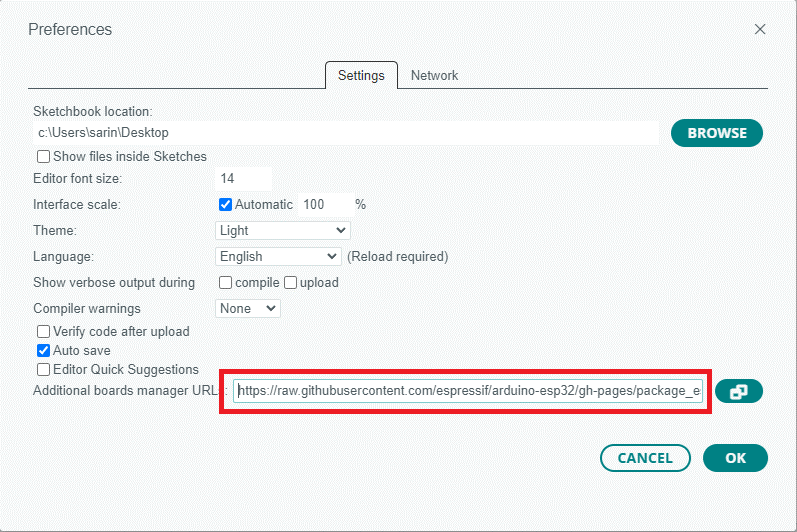
\includegraphics[width=0.75\textwidth]{assets/metodos_herramientas/arduino_placas.png}
    \caption{Selección de placas ESP32 en Arduino IDE.}
    \label{fig:arduino_placas}
\end{figure}

El siguiente paso es instalar los controladores para la placa ESP32, se muestra en la figura  \ref{fig:arduino_install_esp32}.

\begin{figure}[!ht]
    \centering
    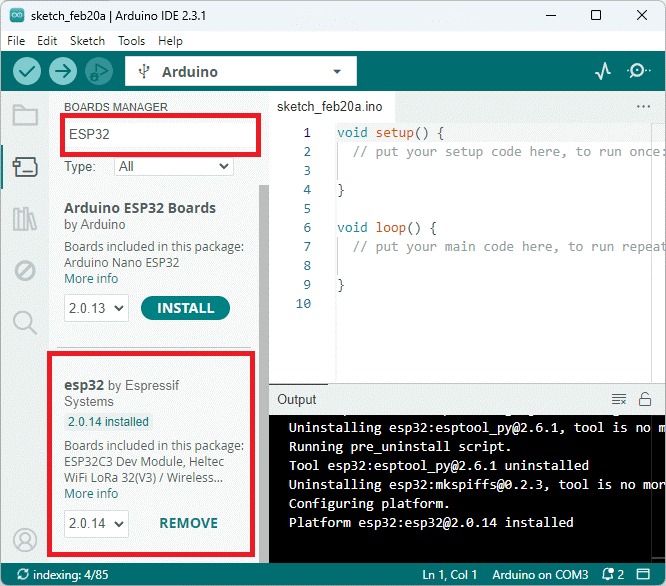
\includegraphics[width=0.75\textwidth]{assets/metodos_herramientas/arduino_install_esp32.png}
    \caption{Instalación del soporte para ESP32 en Arduino IDE.}
    \label{fig:arduino_install_esp32}
\end{figure}

\newpage

Código de prueba:
\begin{lstlisting}[language=C++, label={lst:esp32_blink}, caption={Ejemplo de código de parpadeo de LED en ESP32}]
#include <Arduino.h>
#define LED 2
void setup() {
  Serial.begin(115200);
  pinMode(LED, OUTPUT);
}
void loop() {
  digitalWrite(LED, HIGH);
  delay(1000);
  digitalWrite(LED, LOW);
  delay(1000);
}
\end{lstlisting}

\subsection{Micrófono INMP441}
\begin{figure}[!ht]
    \centering
    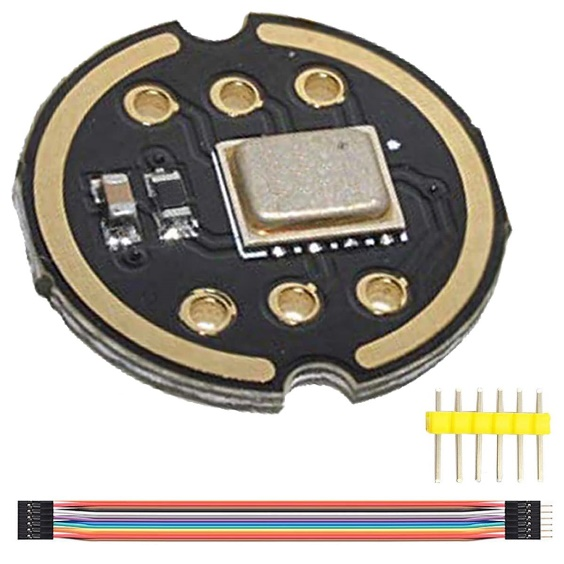
\includegraphics[width=0.75\textwidth]{assets/metodos_herramientas/inmp441.png}
    \caption{Módulo de micrófono INMP441.}
    \label{fig:inmp441}
\end{figure}

El sensor INMP441 es un micrófono multidireccional que utiliza el protocolo I2S~\cite{keysight_i2s_blog} para transferencia de audio, de la misma manera que, y como se mencionó en los trabajos relacionados, el dispositivo INMP401 es utilizado con el controlador ESP8266, el dispositivo INMP441 es comúnmente utilizado con el dispositivo ESP32, principalmente por su compatibilidad mediante el protocolo I2S. El módulo INMP441 se muestra en la figura  7~\cite{inmp441_datasheet}.




\backmatter

\printbibliography[title={REFERENCIAS}]

\end{document}